% Judul dokumen
\title{Buku Tugas Akhir ITS}
\author{Chang, Charles}

% Pengaturan ukuran teks dan bentuk halaman dua sisi
\documentclass[10pt,twoside]{report}

% Pengaturan ukuran halaman dan margin
\usepackage[a5paper,top=25mm,left=25mm,right=20mm,bottom=25mm]{geometry}

% Pengaturan ukuran spasi
\usepackage[singlespacing]{setspace}

% Pengaturan format bahasa
\usepackage[indonesian]{babel}

% Pengaturan jenis karakter
\usepackage[utf8]{inputenc}

% Pengaturan pewarnaan
\usepackage[table,xcdraw]{xcolor}

% Pengaturan kutipan artikel
\usepackage[numbers]{natbib}

% Package lainnya
\usepackage{changepage}
\usepackage{enumitem}
\usepackage{eso-pic}
\usepackage{etoolbox}
\usepackage{graphicx}
\usepackage{lipsum}
\usepackage{lmodern}
\usepackage{longtable}
\usepackage{tabularx}
\usepackage{wrapfig}

\usepackage[hyphens]{url}
% Pengaturan detail pada file PDF
\usepackage[pdfauthor={@author},bookmarksnumbered,pdfborder={0 0 0}, breaklinks]{hyperref}

% Definisi untuk "Hati ini sengaja dikosongkan"
\patchcmd{\cleardoublepage}{\hbox{}}{
  \thispagestyle{empty}
  \vspace*{\fill}
  \begin{center}\textit{[Halaman ini sengaja dikosongkan]}\end{center}
  \vfill}{}{}

% Pengaturan penomoran halaman
\usepackage{fancyhdr}
\fancyhf{}
\renewcommand{\headrulewidth}{0pt}
\pagestyle{fancy}
\fancyfoot[CE,CO]{\thepage}
\patchcmd{\chapter}{plain}{fancy}{}{}
\patchcmd{\chapter}{empty}{plain}{}{}

% Pengaturan format judul bab
\usepackage{titlesec}
\titleformat{\chapter}[display]{\bfseries\Large}{BAB \centering\Roman{chapter}}{0ex}{\vspace{0ex}\centering}
\titleformat{\section}{\bfseries\large}{\MakeUppercase{\thesection}}{1ex}{\vspace{1ex}}
\titleformat{\subsection}{\bfseries\large}{\MakeUppercase{\thesubsection}}{1ex}{}
\titleformat{\subsubsection}{\bfseries\large}{\MakeUppercase{\thesubsubsection}}{1ex}{}
\titlespacing{\chapter}{0ex}{0ex}{4ex}
\titlespacing{\section}{0ex}{1ex}{0ex}
\titlespacing{\subsection}{0ex}{0.5ex}{0ex}
\titlespacing{\subsubsection}{0ex}{0.5ex}{0ex}

% Pengaturan format potongan kode
\usepackage{listings}
\definecolor{comment}{RGB}{0,128,0}
\definecolor{string}{RGB}{255,0,0}
\definecolor{keyword}{RGB}{0,0,255}
\lstdefinestyle{codestyle}{
  commentstyle=\color{comment},
  stringstyle=\color{string},
  keywordstyle=\color{keyword},
  basicstyle=\footnotesize\ttfamily,
  numbers=left,
  numberstyle=\tiny,
  numbersep=5pt,
  frame=lines,
  breaklines=true,
  prebreak=\raisebox{0ex}[0ex][0ex]{\ensuremath{\hookleftarrow}},
  showstringspaces=false,
  upquote=true,
  tabsize=2,
}
\lstset{style=codestyle}

% Isi keseluruhan dokumen
\begin{document}

  % Sampul luar Bahasa Indonesia
  \newcommand\covercontents{sampul/konten-id.tex}
  \AddToShipoutPictureBG*{
  \AtPageLowerLeft{
    % Ubah nilai berikut jika posisi horizontal background tidak sesuai
    \hspace{-3.5mm}

    % Ubah nilai berikut jika posisi vertikal background tidak sesuai
    \raisebox{0mm}{
      
\includegraphics[width=\paperwidth,height=\paperheight]{sampul/gambar/sampul-luar.png}
    }
  }
}

% Menyembunyikan nomor halaman
\thispagestyle{empty}

% Pengaturan margin untuk menyesuaikan konten sampul
\newgeometry{
  top=95mm,
  left=25mm,
  right=20mm,
  bottom=25mm
}

\begin{flushleft}

  % Pemilihan font sans serif
  \sffamily

  % Pemilihan warna font putih
  \color{white}

  % Pemilihan font bold
  \fontseries{bx}
  \selectfont

  \input{\covercontents}

\end{flushleft}

\restoregeometry


  % Atur ulang penomoran halaman
  \setcounter{page}{1}

  % Sampul dalam Bahasa Indonesia
  \renewcommand\covercontents{sampul/konten-id.tex}
  \AddToShipoutPictureBG*{
  \AtPageLowerLeft{
    % Ubah nilai berikut jika posisi horizontal background tidak sesuai
    \hspace{-3.5mm}

    % Ubah nilai berikut jika posisi vertikal background tidak sesuai
    \raisebox{0mm}{
      
\includegraphics[width=\paperwidth,height=\paperheight]{sampul/gambar/sampul-dalam.png}
    }
  }
}

% Menyembunyikan nomor halaman
\thispagestyle{empty}

% Pengaturan margin untuk menyesuaikan konten sampul
\newgeometry{
  top=95mm,
  left=25mm,
  right=20mm,
  bottom=25mm
}

\begin{flushleft}

  % Pemilihan font sans serif
  \sffamily

  % Pemilihan font bold
  \fontseries{bx}
  \selectfont

  \input{\covercontents}

\end{flushleft}

\restoregeometry

  \clearpage
  \cleardoublepage

  % Sampul dalam Bahasa Inggris
  \renewcommand\covercontents{sampul/konten-en.tex}
  \AddToShipoutPictureBG*{
  \AtPageLowerLeft{
    % Ubah nilai berikut jika posisi horizontal background tidak sesuai
    \hspace{-3.5mm}

    % Ubah nilai berikut jika posisi vertikal background tidak sesuai
    \raisebox{0mm}{
      
\includegraphics[width=\paperwidth,height=\paperheight]{sampul/gambar/sampul-dalam.png}
    }
  }
}

% Menyembunyikan nomor halaman
\thispagestyle{empty}

% Pengaturan margin untuk menyesuaikan konten sampul
\newgeometry{
  top=95mm,
  left=25mm,
  right=20mm,
  bottom=25mm
}

\begin{flushleft}

  % Pemilihan font sans serif
  \sffamily

  % Pemilihan font bold
  \fontseries{bx}
  \selectfont

  \input{\covercontents}

\end{flushleft}

\restoregeometry

  \cleardoublepage

  % Pengaturan ukuran indentasi paragraf
  \setlength{\parindent}{2em}

  % Pengaturan ukuran spasi paragraf
  \setlength{\parskip}{1ex}

  % Pernyataan keaslian
  \begin{center}
  \large
  \textbf{PERNYATAAN KEASLIAN\\TUGAS AKHIR}
\end{center}

% Menyembunyikan nomor halaman
\thispagestyle{empty}

\vspace{2ex}

% Ubah paragraf-paragraf berikut sesuai dengan yang ingin diisi pada pernyataan keaslian

Dengan ini saya menyatakan bahwa isi buku Tugas Akhir saya dengan judul “Re-identifikasi Orang menggunakan Lightweight Convolutional Neural Network pada Multi-Modal Image” adalah benar-benar hasil karya intelektual sendiri, diselesaikan tanpa menggunakan bahanbahan yang tidak diizinkan dan bukan merupakan karya orang lain yang saya akui sebagai karya sendiri.

Semua referensi yang dikutip maupun dirujuk telah ditulis secara lengkap pada daftar pustaka.

Apabila ternyata pernyataan ini tidak benar, saya bersedia menerima
sanksi sesuai dengan peraturan yang berlaku.

\vspace{4ex}

\begin{flushright}
  \begin{tabular}[b]{c}
    % Ubah kalimat berikut sesuai dengan tempat, bulan, dan tahun penulisan
    Surabaya, Mei 2021\\
    \\
    \\
    \\
    \\
    % Ubah kalimat-kalimat berikut sesuai dengan nama dan NRP mahasiswa
    Charles Chang\\
    07211740000027
  \end{tabular}
\end{flushright}

  \cleardoublepage

  % Lembar pengesahan
  \begin{center}
	\large
  \textbf{LEMBAR PENGESAHAN}
\end{center}

% Menyembunyikan nomor halaman
\thispagestyle{empty}

\begin{center}
  % Ubah kalimat berikut dengan judul tugas akhir
  \textbf{Re-identifikasi Orang menggunakan
  	Lightweight Convolutional Neural Network pada Multi-Modal Image}
\end{center}

\begingroup
  % Pemilihan font ukuran small
  \small

  \begin{center}
    % Ubah kalimat berikut dengan pernyataan untuk lembar pengesahan
    Tugas Akhir ini disusun untuk memenuhi salah satu syarat memperoleh
    gelar Sarjana Teknik di Institut Teknologi Sepuluh Nopember Surabaya
  \end{center}

  \begin{center}
    % Ubah kalimat berikut dengan nama dan NRP mahasiswa
    Oleh: Charles Chang (NRP. 07211740000027)
  \end{center}

  \begin{center}
    % Ubah kalimat-kalimat berikut dengan tanggal ujian dan periode wisuda
    Tanggal Ujian : Kamis 22 Juli 2021\\
    Periode Wisuda : September 2021
  \end{center}

  \begin{center}
    Disetujui Oleh:
  \end{center}

  \begingroup
    % Menghilangkan padding
    \setlength{\tabcolsep}{0pt}

    \noindent
    \begin{tabularx}{\textwidth}{X c}
      % Ubah kalimat-kalimat berikut dengan nama dan NIP dosen pembimbing pertama
      Dr. Reza Fuad Rachmadi, S.T., M.T. & (Pembimbing I) \\
      NIP: 19850403 201212 1 001        &  \\
      &  \\
      &  \\
      % Ubah kalimat-kalimat berikut dengan nama dan NIP dosen pembimbing kedua
      Dr. I Ketut Eddy Purnama, S.T, M.T.  & (Pembimbing II) \\
      NIP: 19690730 199512 1 001        &  \\
      &  \\
      &  \\
      % Ubah kalimat-kalimat berikut dengan nama dan NIP dosen penguji pertama
      Eko Pramunanto S.T., M.T.  & (Penguji I) \\
      NIP: 196612031994121001        &  \\
      &  \\
      &  \\
      % Ubah kalimat-kalimat berikut dengan nama dan NIP dosen penguji kedua
      Arief Kurniawan S.T. M.T.  & (Penguji II) \\
      NIP: 197409072002121001        & \\
      &  \\
      &  \\
      % Ubah kalimat-kalimat berikut dengan nama dan NIP dosen penguji ketiga
      Dion Hayu Fandiantoro, S.T., M.Eng. & (Penguji III) \\
      NIP: 1994202011064       & \\
    \end{tabularx}
  \endgroup

  \vspace{2ex}

  \begin{center}
    % Ubah kalimat berikut dengan jabatan kepala departemen
    Mengetahui, \\
    Kepala Departemen Teknik Komputer - ITS \\

    \vspace{8ex}

    % Ubah kalimat-kalimat berikut dengan nama dan NIP kepala departemen
    \underline{Dr. Supeno Mardi Susiki Nugroho, ST., MT.} \\
    NIP. 19700313 199512 1 001
  \end{center}
\endgroup

  \cleardoublepage

  % Nomor halaman pembuka dimulai dari sini
  \pagenumbering{roman}

  % Abstrak Bahasa Indonesia
  \begin{center}
	\Large\textbf{ABSTRAK}
\end{center}
\vspace{1ex}

\begin{adjustwidth}{-0.2cm}{}
	\begin{tabular}{lcp{0.6\linewidth}}
		Nama Mahasiswa &:& Charles Chang \\
		Judul Tugas Akhir &:& Re-identifikasi Orang menggunakan
		Lightweight Convolutional Neural Network
		pada Multi-Modal Image\\
		Pembimbing &:& 1. Dr. Reza Fuad Rachmadi, S.T., M.T. \\
		& & 2. Dr. I Ketut Eddy Purnama, S.T, M.T.  \\
	\end{tabular}
\end{adjustwidth}
\vspace{1ex}

\setlength{\parindent}{0cm} Sebagai alat pelengkap keamanan, sistem CCTV semakin banyak digunakan di setiap ruang publik untuk memantau dan menganalisa tindakan kriminal pada suatu lokasi. Akan tetapi, pencarian kriminal secara manual masih rentan akan kesalahan manusia. Salah satu solusi membuat pencarian kriminal lebih efektif dan efisien adalah dengan penggunaan Re-identifikasi.
\par  Re-identifikasi merupakan sebuah teknik visi komputer dan deep learning dimana dilakukan pencarian ulang citra atau video milik sebuah identitas.Pada tugas akhir ini, akan dipelajari metode Re-identifikasi orang dengan citra multi-modal, adapun data Input yang akan digunakan berupa sketsa tubuh yang digambar oleh beberapa seniman berbeda.
\par  Teknik yang dipelajari akan diimplementasikan menggunakan Lightweight Convolutional Neural Network dan pre-trained weights dari model yang digunakan untuk mengklasifikasi dataset CIFAR-10. Hasil yang diharapkan melalui Tugas Akhir ini adalah terciptanya sebuah model yang dapat melakukan Re-identifikasi orang riil dari input sketsa menggunakan Lightweight Convolutional Neural Network, sehingga pencarian kriminal di Indonesia dapat dilakukan dengan lebih efisien. Pada penelitian ini kami mendapatkan akurasi Rank-1 sebesar 21\% dengan menggunakan model ensemble kami, serta mendapatkan akurasi Rank-1 sebesar 19.8\% dengan menggunakan model ResNet110.

\vspace{2ex}

Kata Kunci : Re-identifikasi, Multi-Modal, Kriminal
\newpage
  \cleardoublepage

  % Abstrak Bahasa Inggris
  \begin{center}
  \large\textbf{ABSTRACT}
\end{center}

\addcontentsline{toc}{chapter}{ABSTRACT}

\vspace{2ex}

\begingroup
  % Menghilangkan padding
  \setlength{\tabcolsep}{0pt}

  \noindent
  \begin{tabularx}{\textwidth}{l >{\centering}m{3em} X}
    % Ubah kalimat berikut dengan nama mahasiswa
    \emph{Name}     &:& Charles Chang \\

    % Ubah kalimat berikut dengan judul tugas akhir dalam Bahasa Inggris
    \emph{Title}    &:& \emph{Multi-Modal Person Re-Identification using Lightweight Convolutional Neural Network} \\

    % Ubah kalimat-kalimat berikut dengan nama-nama dosen pembimbing
    \emph{Advisors} &:& 1. Dr. Reza Fuad Rachmadi, S.T., M.T. \\
                    & & 2. Dr. I Ketut Eddy Purnama, S.T, M.T \\
  \end{tabularx}
\endgroup

% Ubah paragraf berikut dengan abstrak dari tugas akhir dalam Bahasa Inggris
\emph{As a complement to security systems, CCTVs are increasingly used to monitor and analyze criminal acts done at a given location. However, the manual search for criminals is still prone to human error. One of the solutions to make the process more effective and efficient is with the use of re-identification.}

\emph{Re-identification is a computer vision and deep learning technique in which an anonymized identity of an image is matched with its owner. In this paper, we will study the method of re-identifying people with multi-modal images where the query is in the form of a body sketch drawn by several different artists.}

\emph{Re-identification techniques in this book are implemented using lightweight Convolutional Neural Network, namely the Residual Network used to classify the CIFAR10 dataset. In this research, we achieved a Rank-1 accuracy of 21\% with our ensemble model, and 19.8 \% with our ResNet 110 model.}

% Ubah kata-kata berikut dengan kata kunci dari tugas akhir dalam Bahasa Inggris
\emph{Keywords}: \emph{Re-Identification}, \emph{Multi-Modal}, \emph{Criminal}.

  \cleardoublepage

  % Kata pengantar
  \begin{center}
	\Large\textbf{KATA PENGANTAR}
\end{center}
\vspace{1ex}

\setlength{\parindent}{0.9cm} Puji dan syukur kehadirat Tuhan Yang Maha Esa atas segala karunia-Nya, penulis  dapat menyelesaikan penelitian ini dengan judul \textbf{Re-identifikasi Orang menggunakan Lightweight Convolutional Neural Network pada Multi-Modal Image}.
\vspace{1ex}

Penelitian ini disusun dalam rangka pemenuhan bidang riset di Departemen Teknik Komputer ITS, Bidang Studi \textit{Telematika}, serta digunakan sebagai persyaratan menyelesaikan pendidikan  S1. Oleh karena itu, penulis mengucapkan terima kasih kepada:
\vspace{1ex}

\begin{enumerate}[nolistsep]
	\item Tuhan Yang Maha Esa
	\item Orang tua saya, atas semangat dan segala dukungan yang telah diberikan
	\item Bapak Dr. Reza Fuad Rachmadi, S.T., M.T.
	\item Bapak Dr. I Ketut Eddy Purnama, S.T, M.T.
	\item Bapak-ibu dosen pengajar Departemen Teknik Komputer, atas pengajaran, bimbingan, serta perhatian yang diberikan kepada penulis selama ini.
	\item Sesama asisten lab B201 yang menemani pengerjaan Tugas Akhir.
	\item Serta teman - teman angkatan 2017 yang telah bersama - sama melalui kehidupan perkuliahan bersama penulis
\end{enumerate}
\vspace{1ex}

Kesempurnaan hanya milik Tuhan Yang Maha Esa, untuk itu penulis memohon segenap kritik dan saran yang  membangun. Semoga penelitian ini dapat memberikan manfaat bagi kita semua. Amin.
\begin{flushright}
	\begin{tabular}[b]{c}
		Surabaya, April 2021
		\\
		\\
		Penulis
	\end{tabular}
\end{flushright}
  \cleardoublepage

  % Daftar isi
  \renewcommand*\contentsname{DAFTAR ISI}
  \addcontentsline{toc}{chapter}{\contentsname}
  \tableofcontents
  \cleardoublepage

  % Daftar gambar
  \renewcommand*\listfigurename{DAFTAR GAMBAR}
  \addcontentsline{toc}{chapter}{\listfigurename}
  \listoffigures
  \cleardoublepage

  % Daftar tabel
  \renewcommand*\listtablename{DAFTAR TABEL}
  \addcontentsline{toc}{chapter}{\listtablename}
  \listoftables
  \cleardoublepage

  % Nomor halaman isi dimulai dari sini
  \pagenumbering{arabic}

  % Bab 1 pendahuluan
  \chapter{PENDAHULUAN}
\pagenumbering{arabic}
\vspace{1ex}

\section*{}
Penelitian ini di latar belakangi oleh berbagai kondisi yang menjadi acuan. Selain itu juga terdapat beberapa permasalahan yang akan dijawab sebagai luaran dari penelitian.
\vspace{1ex}

\section{Latar belakang}
\vspace{1ex}

Re-identifikasi manusia merupakan sebuah teknik visi komputer dan deep learning dimana pada sebuah lingkungan yang terdapat beberapa kamera pengawas dilakukan adanya pencocokan citra seseorang, kepada citra yang ditangkap pada kamera lain. Masalah utama yang ditangani oleh Re-identifikasi manusia dapat disimpulkan sebagai cara untuk mencari representasi diskriminatif milik individu yang ingin dicari. Dengan membuat sistem re-identifikasi manusia, pemeriksaan hasil rekaman yang dilakukan oleh pihak kepolisian dapat dilakukan dengan jauh lebih cepat, dan dapat menekan biaya yang digunakan untuk membayar tenaga kerja. Tidak hanya  untuk melakukan pencarian pelaku tindak kriminal, re-identifikasi dapat digunakan juga untuk melihat apakah barang yang tertinggal pada suatu lokasi diambil individu yang sama, dan dapat membantu pihak sekuriti mencari orang yang hilang. Re-identifikasi manusia dapat mempermudah aktivitas - aktivitas yang sebelumnya dilakukan secara manual, maka dari itu pencarian individu sangat dibutuhkan dengan menggunakan teknologi \textit{machine learning} untuk mempercepat proses yang sebelumnya memakan waktu yang sangat lama.

Namun untuk melakukan re-identifikasi manusia dibutuhkan citra dari pelaku, yang tidak selalu siap tersedia dimiliki oleh pihak kepolisian. Maka dari itu diperlukan adanya re-identifikasi yang menggunakan sketsa sebagai input dari model. Meskipun memiliki konsep yang mirip dengan \textit{Face Recognition}, dikarenakan re-identifikasi sketsa menggunakan gambar \textit{full-body}, terdapat tambahan kompleksitas yang harus dihadapi oleh model yang dibuat. Selain itu masalah ini sangat menantang dikarenakan sketsa tidak memiliki warna sehingga informasi yang didapatkan oleh model lebih sedikit dibanding pada re-identifikasi manusia. 

Penelitian ini telah dilakukan sebelumnya oleh Lu Pang et al. dengan menggunakan model yang canggih dan \textit{cross-domain adversarial learning}, dimana model yang dibuat dapat mencapai Rank-1 akurasi sebesar 34\%. Pada penelitian ini dataset yang digunakan merupakan dataset satu-satunya yang tersedia untuk melakukan re-identifikasi sketsa, yaitu PKU Sketch Re-ID, sebuah dataset yang memuat 200 individu, dimana setiap individu memiliki 3 buah citra, yaitu dua buah citra CCTV dan sebuah citra sketsa. Dataset ini merupakan dataset yang sangat kecil apabila dibandingkan dengan dataset-dataset Person Re-Identification lainnya. Sebagai contoh, dataset Market-1501 memiliki total citra reidentifikasi sebanyak 15535 citra, yaitu 25.8 kali lebih banyak dibandingkan data yang dimiliki oleh dataset PKU Sketch Re-ID. Dikarenakan keterbatasan data yang dimiliki oleh dataset PKU Sketch Re-ID, dataset satu-satunya yang menggunakan citra sketsa \textit{full-body} sebagai input dari model, re-identifikasi sketsa ke manusia masih sangat sulit untuk dilakukan. 

Selain itu penelitian lebih lanjut menggunakan model \textit{lightweight} masih belum pernah dilakukan. Penggunaan model lightweight sangatlah berguna pada kasus \textit{Edge Computing} dimana komputasi dilakukan sedekat mungkin dengan pengguna, sehingga mengurangi waktu respon dan menghemat \textit{bandwidth}. Pada umumnya untuk mengolah data yang sangat besar seperti data dari CCTV dengan cepat, dibutuhkan sebuah server pusat yang sangat dekat dengan pengguna untuk mengatasi isu latensi, namun dengan adanya edge computing, pihak kepolisian dari masing-masing daerah dapat melakukan re-identifikasi pada \textit{edge data center} yang tersedia pada daerahnya. Sehingga dapat menghindari resiko \textit{downtime} maupun latensi yang terjadi apabila komputasi dilakukan pada server pusat.

\pagebreak

Namun Edge Computing tidak lepas dari kekurangan, dikarenakan dilakukan sedekat mungkin dengan pengguna, kekuatan perangkat pada Edge Computing sangatlah terbatas. Dibutuhkan sebuah model \textit{lightweight} sehingga model dapat di jalankan pada perangkat yang memiliki kekuatan komputasi yang tidak terlalu besar. 

Oleh karena itu, pada penelitian ini kami memilih untuk menggunakan model \textit{lightweight}. Model \textit{lightweight} yang kami gunakan merupakan model Residual Network CIFAR-10 dimana Fully Connected layer terakhir dihapus, dan ditambahkan dua buah Fully-Connected layer baru dengan konfigurasi berbeda dengan Fully-Connected layer yang sebelumnya. 

Dengan adanya penelitian ini, diharapkan hasil re-identifikasi sketsa dapat diolah dan dikembangkan untuk membantu pencarian pelaku tindak kriminal oleh pihak kepolisian di Indonesia.

\vspace{1ex} 
\section{Permasalahan}
\vspace{1ex}
Berdasarkan data yang telah dipaparkan di latar belakang, dapat dirumuskan beberapa rumusan masalah sebagai berikut:
\begin{enumerate}
	\vspace{-1.3mm}
	\item Data hasil rekaman kamera masih diperiksa secara manual oleh pihak kepolisian, dari data yang diambil dari Kedeputian Pelayanan Publik Indonesia, dibutuhkan waktu 8 jam untuk melakukan pengecekan sebuah rekaman CCTV \cite{cit:3}. Oleh karena itu dibutuhkan metode pengecekan yang lebih cepat.
	\vspace{-2mm}
	\item Dataset PKU Sketch Re-ID yang digunakan memiliki jumlah data yang relatif sedikit. Jumlah total citra yang dimiliki oleh PKU Sketch Re-ID hanyalah 3.86\% dari total citra dataset Market 1501, dataset yang sangat umum digunakan untuk re-identifikasi sketsa.
	\vspace{-2mm}
	\item Dikarenakan terdapat perbedaan modalitas pada citra sketsa dan citra CCTV, dimana intepretasi citra sketsa masing-masing individu berbeda-beda dikarenakan dilukis oleh seniman yang berbeda beda. Selain itu, sketsa yang digunakan, tidak memiliki warna, sehingga fitur yang dapat digunakan oleh model untuk melakukan re-identifikasi hanyalah fitur tekstur dan warna.
	\vspace{-2mm}
	\item Dibutuhkan sebuah metode yang dapat melakukan re-identifikasi dengan cepat dan tidak membutuhkan kekuatan komputasi yang besar sehingga dapat digunakan pada \textit{edge computing} atau pada \textit{end device}.
\end{enumerate}

\section{Tujuan}
\vspace{1ex}

Adapun tujuan dari penelitian Tugas Akhir ini adalah mengembangkan model re-identifikasi orang menggunakan \textit{Lightweight Convolutional Neural Network}, guna menghasilkan model re-identifikasi sketsa yang lebih efisien akan kekuatan komputasi, sehingga dapat digunakan pada Edge Computing.

\vspace{1ex}

\section{Batasan masalah}
\vspace{1ex}
Batasan masalah yang timbul dari permasalahan Tugas Akhir ini adalah:
\vspace{1ex}
\begin{enumerate}
	\vspace{-2mm}
	\item Data \textit{training} dan \textit{testing} menggunakan data yang diambil dari PKU SketchRe-ID Dataset.
	\vspace{-2mm}
	\item Jenis re-identifikasi orang yang akan dilakukan adalah \textit{Closed Set} dan \textit{Short Term}, dimana dataset tetap dan tidak bertambah seiring dengan waktu.
	\vspace{-2mm}
	\item Training akan dilakukan menggunakan \textit{Lightweight Convolutional Neural Network} sehingga dapat mengurangi kekuatan komputasi yang dibutuhkan oleh model.
\end{enumerate}
\vspace{1ex}

\section{Manfaat}
\vspace{1ex}
Manfaat dari Tugas Akhir ini sendiri adalah, untuk mempercepat pencarian pelaku tindak kriminal dimana citra milik pelaku tidak dimiliki, sehingga digunakan input sketsa. Selain itu model yang digunakan pada Tugas Akhir ini merupakan model \textit{lightweight}, yang sangat berguna pada rana \textit{Edge Computing}, dimana kekuatan komputasi terbatas.
  \cleardoublepage

  % Bab 2 tinjauan pustaka
  \chapter{TINJAUAN PUSTAKA}
\vspace{1ex}

\section{\textit{State of the Art}}
\begin{enumerate}
	\item Lightweight Residual Network for Person Re-Identification (Reza Fuad Rachmadi, Supeno Mardi Nugroho, I Ketut Eddy Purnama) \cite{cit:14}
	\par
	\textit{Lightweight Residual Network for Person Re-Identification} ini merupakan sebuah implementasi \textit{lightweight CNN} untuk melakukan re-Identifikasi manusia, lightweight CNN yang digunakan berbasis \textit{Residual Network} dengan menggunakan pre trained weights yang pernah  digunakan untuk memecahkan masalah klasifikasi CIFAR-10. Berdasarkan hasil dari riset yang dilakukan, meskipun lightweight CNN tidak mendapatkan akurasi tercanggih dibandingkan model-model lainnya, banyak nya informasi yang didapatkan oleh model ini sangat tinggi, dan dapat dikatakan model ini lebih efisien dari model-model lainnya.
	\vspace{1ex}
	
	\item Torchreid: A Library for Deep Learning Person Re-Identification in Pytorch. (Kaiyang Zhou, Tao Xiang). \cite{cit:16}
	\par
	Torchreid merupakan sebuah \textit{library deep learning} yang dibuat oleh Kaiyang Zhou untuk mempercepat implementasi dan percobaan re-identifikasi. Library ini secara umum dibuat dengan menggunakan bahasa Python dengan beberapa kode berbasis Cython untuk optimisasi. Pada library ini dataset sudah di \textit{preprocess} dan di implementasi sesuai dengan protokol evaluasi masing masing dataset sehingga dapat dibandingkan dengan penelitian lain yang terkait.
	\vspace{1ex}
	
	\pagebreak
	
	\item Adaptive L2 Regularization in Person Re-Identification. (Xingyang Ni, Liang Fang, Heikki Huttunen) \cite{cit:17}
	\par
	
	\textit{Adaptive L2 Regularization in Person Re-Identication} merupakan sebuah penelitian untuk menambahkan regularisasi L2, dimana faktor regularisasi dapat berubah ubah secara adaptif pada \textit{baseline} model. Dari hasil penelitan yang dilakukan regularisasi L2 secara adaptif dapat meningkatkan akurasi model sekitar 1 hingga 2\% untuk \textit{dataset} Market-1501, DukeMTMC dan MSMT17.
	\vspace{1ex}
	
	\item Cross-Domain Adversarial Feature Learning for Sketch
	Re-identification. (Lu Pang, Yaowei Wang, Yi-Zhe Song, Tiejun Huang, Yonghong Tian) \cite{cit:12}
	\par
	
	\textit{Cross-Domain Adversarial Feature Learning for Sketch Re-identification} merupakan penelitian yang pertama kali menggunakan gambar sketsa sebagai input dari model re-identifikasi manusia, namun dari model yang digunakan sendiri merupakan model yang telah di optimisasi untuk melakukan pengambilan informasi dari sketsa, seperti Triplet SN dan model GN Siamese yang merupakan gabungan dari dua cabang dari model GoogleNet yang dioptimisasi dengan menggunakan pairwise verification loss.
	\vspace{1ex}
	
\end{enumerate}
\par Dapat dilihat dari penelitian-penelitian terkait diatas, selain pada penelitian \textit{Cross-Domain Adversarial Feature Learning for Sketch Re-identification}, fokus dari permasalahan adalah penggunaan metode re-identifikasi pada citra manusia yang tertangkap pada CCTV. Sedangkan pada penelitian yang kami usulkan merupakan implementasi re-identifikasi pada citra orang riil yang tertangkap pada CCTV, menggunakan citra sketsa \textit{full body} sebagai \textit{input}.
Selain itu penelitian yang dilakukan menggunakan model \textit{lightweight classical} seperti ResNet, yang bukan merupakan fokus dari penelitian \textit{Cross-Domain Adversarial Feature Learning for Sketch Re-identification}.
\vspace{1ex}

\section*{}
Demi mendukung penelitian ini, dibutuhkan beberapa teori penunjang sebagai bahan acuan dan referensi. Dengan demikian penelitian ini menjadi lebih terarah. 
\vspace{1ex}

\section{Machine Learning}
\vspace{1ex}

\begin{figure} [!htb]
	\centering
	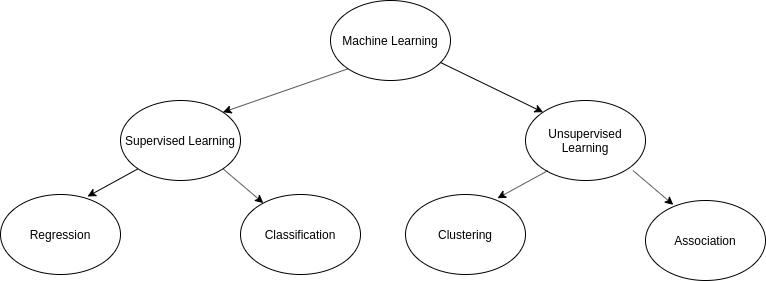
\includegraphics[scale=0.28]{img/machinelearning.png}
	\caption{Jenis Machine Learning}
	\label{fig:2.0}
\end{figure}

\textit{Machine learning} atau pembelajaran mesin adalah suatu cabang teknologi yang menerapkan penggunaan \textit{artificial intelligence}. \textit{Machine learning} pertama kali diperkenalkan oleh Thomas Bayes, Adrien-Marie Legendre, dan Andrey Markov pada sekitar tahun 1920\cite{cit:7}. Dengan berkembangnya \textit{machine learning}, tugas-tugas yang dilakukan oleh \textit{machine learning} ini pun semakin beragam, dimana secara umum jenis pembelajaran pada Machine Learning dapat dikelompokkan menjadi dua, yaitu Supervised Learning dan Unsupervised Learning.

\vspace{1ex}
\par \textit{Supervised learning} jika diartikan secara harfiah adalah pembelajaran yang ada supervisornya. Disini supervisi dilakukan oleh orang yang melakukan training kepada label di setiap datanya. Sebagai contoh dapat dilihat pada gambar \ref{fig:2.1}. 
\vspace{1ex}

\begin{figure} [!htb]
	\centering
	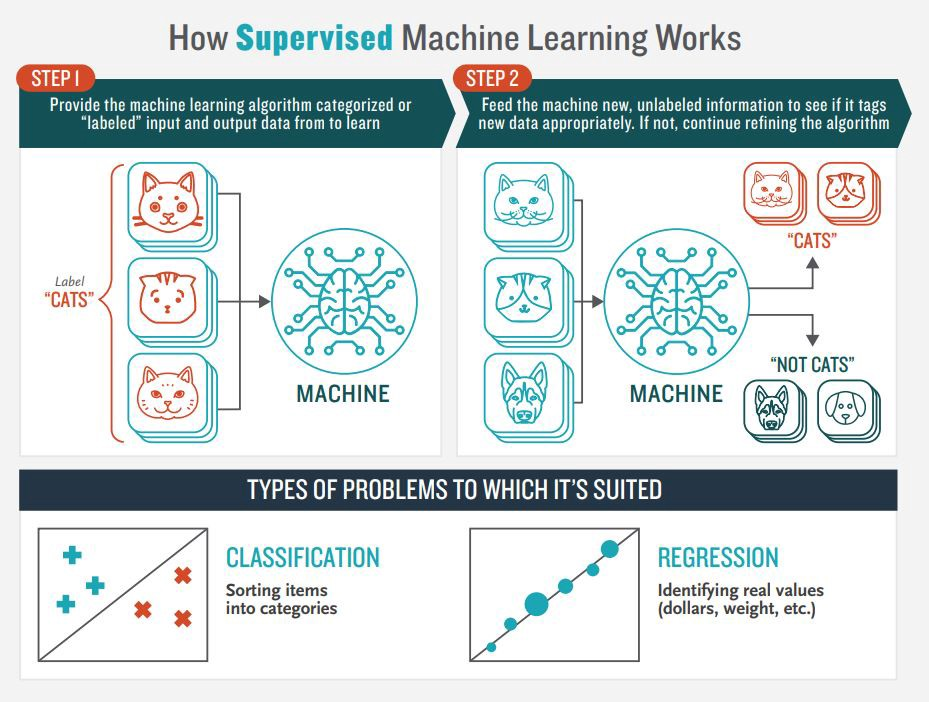
\includegraphics[scale=0.16]{img/supervised.jpeg}
	\caption{Cara Kerja Supervised Learning\cite{cit:8}}
	\label{fig:2.1}
\end{figure}

\par Pada gambar diatas, masing-masing gambar kucing diberi label “CATS” dan yang bukan kucing (“anjing”,”beruang”,”lain-lain”) diberi label “NOT CATS”. Ketika gambar baru dimasukkan setiap label akan dicompare sampai selesai, dan yang memiliki persentase lebih banyak akan diambil sebagai prediksi akhir.

\vspace{1ex}

\par Pada pendekatan \textit{supervised learning}, terdapat input dan output yang dibuat menjadi hubungan matematis. \textit{Supervised learning} cocok untuk digunakan untuk memprediksi dimana sudah ada contoh data yang lengkap, sehingga pola yang terbentuk adalah hasil pembelajaran dari data lengkap tersebut. Beberapa algoritma yang termasuk dalam \textit{supervised learning} adalah sebagai berikut:
\begin{enumerate}
	\vspace{-2mm}
	\item Regresi Linier Berganda
	\vspace{-2mm}
	\item Analisis Deret Waktu
	\vspace{-2mm}
	\item \textit{Decision Tree} dan \textit{Random Forest}
	\vspace{-2mm}
	\item \textit{Naive Bayes Classifier}
	\vspace{-2mm}
	\item \textit{Nearest Neighbor Classifier}
	\vspace{-2mm}
	\item \textit{Artificial Neural Network}
	\vspace{-1mm}
\end{enumerate}
\par Jika dibandingkan dengan \textit{supervised learning}, \textit{unsupervised learning} tidak membutuhkan adanya label sebagai dasar prediksi melainkan menggunakan kesamaan atribut - atribut yang dimiliki oleh data tersebut. Jika atribut - atribut tersebut memiliki kesamaan maka data tersebut akan di \textit{cluster} menjadi satu. Sebagai contoh dapat dilihat pada gambar \ref{fig:Unsupervised} :

\begin{figure}[h!]
	\centering
	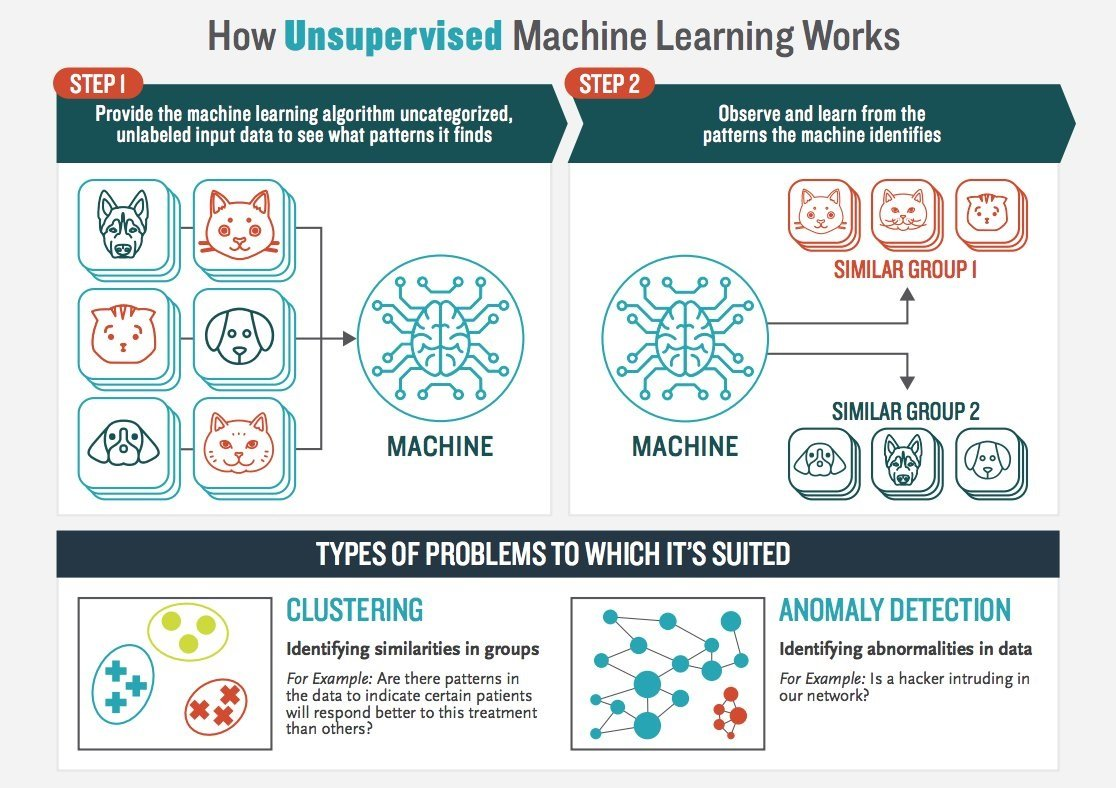
\includegraphics[scale=0.18]{img/unsupervised.jpg}
	\caption{Cara kerja Unsupervised Learning \cite{cit:8}}
	\label{fig:Unsupervised}
\end{figure}

\pagebreak

\par Pada Gambar \ref{fig:Unsupervised} dapat dilihat bahwa disediakan gambar- gambar yang tidak memiliki label ke algoritma \textit{machine learning}. Setelah itu \textit{artificial intelligence} akan memisahkan gambar mana yang memiliki kesamaan di dalam \textit{cluster}. \textit{Cluster} yang ada merupakan hasil akhir klasifikasi yang dilakukan.

\par Namun \textit{unsupervised learning} tidak memiliki hasil spesifik layaknya pada \textit{supervised learning}. Hal ini dikarenakan tidak adanya label dasar (ground truth). Beberapa algoritma yang digunakan di \textit{unsupervised learning} :
\begin{enumerate}
	\vspace{-2mm}
	\item \textit{Clustering}
	\vspace{-2mm}
	\item \textit{Anomaly Detection}
	\vspace{-2mm}
	\item \textit{Training Model}
	\vspace{-2mm}
	\item \textit{Association Discovery}
\end{enumerate}

\vspace{1ex}

\par \textit{Deep learning} (Pembelajaran Dalam) merupakan bagian yang dalam dari \textit{machine learning} yang terdiri dari pemodelan fungsi yang ditata berlapis dan mendalam dengan menggunakan \textit{Artificial Neural Network} (ANN). ANN merupakan sebuah teknik atau pendekatan pengolahan informasi yang terinspirasi oleh cara kerja sistem saraf biologis, khususnya pada sel otak manusia dalam memproses informasi. Jenis pembelajaran dalam deep learning berupa \textit{supervised, semi-supervised}, dan \textit{unsupervised}. Deep learning dapat diimplementasikan dalam pengenalan citra, pengenalan suara, klasifikasi teks, dan sebagainya.

\section{Convolutional Neural Network}
\vspace{1ex}

\begin{figure}[h!]
	\centering
	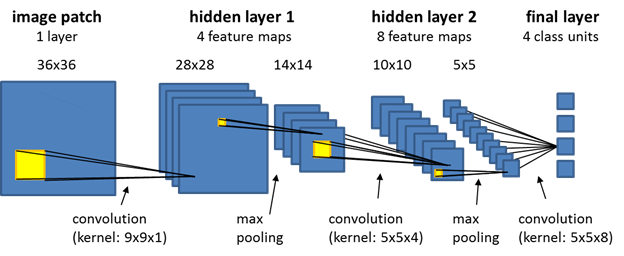
\includegraphics[scale=0.55]{img/CNN_scheme.png}
	\caption{Convolutional Neural Network}
	\label{fig:Convolutional Neural Network}
\end{figure}


Convolutional Neural Network merupakan salah satu algoritma \textit{Deep Learning} yang umum digunakan untuk data berbentuk citra. Convolutional Neural Network memiliki kedalaman yang cukup tinggi sehingga termasuk dalam jenis \textit{Deep Neural Network}. Pada umumnya CNN tidak jauh berbeda dengan neural network pada umumnya, CNN terdiri dari neuron yang memiliki \textit{weight, bias}, dan \textit{activation function}. Dimana weight dari CNN sendiri didapatkan dari persamaan sebagai berikut

\[neuron_{input} \times neuron_{output} \times tinggi \times lebar\] 

Pada Convolutional Neural Network, operasi yang paling utama merupakan Convolutional Layer, dimana terjadi operasi konvolusi pada \textit{output} dari \textit{layer} sebelumnya. Operasi konvolusi merupakan aplikasi kernel pada citra di semua offset sehingga citra secara keseluruhan diubah. Tujuan dari dilakukannya konvolusi itu sendiri adalah untuk melakukan ekstraksi dari fitur-fitur milik citra input.

\section{\textit{Triplet Loss}}
\vspace{1ex}

\begin{figure}[h!]
	\centering
	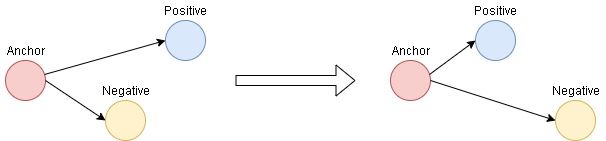
\includegraphics[scale=0.4]{img/TripletLoss.png}
	\caption{Triplet Loss}
	\label{fig:Triplet}
\end{figure}

\par \textit{Triplet Loss} merupakan sebuah \textit{Loss Function} yang umumnya digunakan dalam proses Re-Identifikasi. Pada fungsi ini dilakukan perbandingan jarak antara titik acuan terhadap titik positif yang merupakan gambar dalam kelas sama, dan perbandingan dengan titik negatif yang berasal dari kelas berbeda. Fungsi ini memastikan bahwa jarak ke titik positif akan lebih dekat dibandingkan dengan titik negatif.

\section{CycleGAN}
\vspace{1ex}

\begin{figure}  [!htb]
	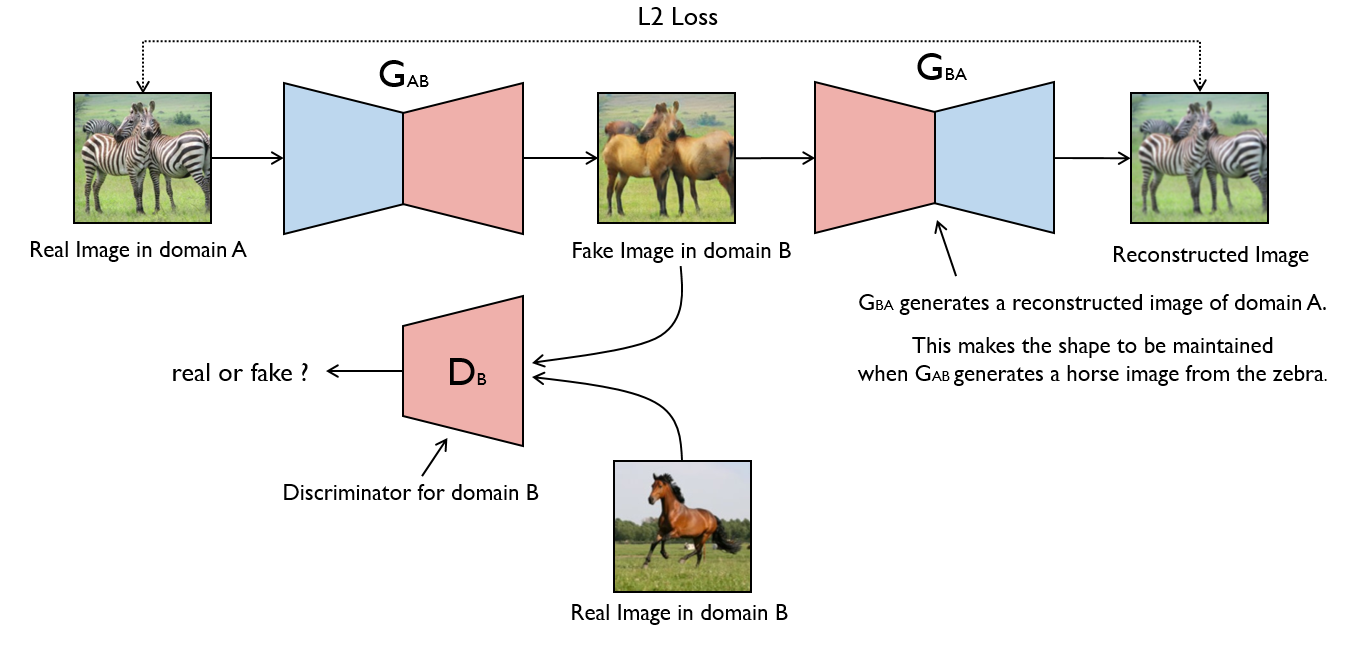
\includegraphics[scale=0.2]{img/cyclegan.png}
	%\caption{Diagram alur kerja}
	\caption{CycleGAN}
	\label{fig: 3_27}
\end{figure}

CycleGAN merupakan sebuah teknik yang menggunakan \textit{Deep Convolutional Neural Network} untuk melakukan sinstesis sebuah gambar versi baru dengan modifikasi yang diinginkan, seperti mengubah gambar dari musim panas ke musim salju. Pada umumnya \textit{training} model untuk melakukan hal tersebut membutuhkan dataset dengan contoh berpasangan(\textit{paired example}) yang sangat besar. Cara seperti ini membutuhkan waktu yang sangat lama, dan pada beberapa kasus tertentu tidak dapat dilakukan. Namun dengan menggunakan CycleGAN, model dapat secara otomatis melakukan \textit{training} untuk translasi \textit{Image-to-image}.  dilatih secara \textit{unsupervised} dengan menggunakan kumpulan gambar dari sebuah domain X ke sebuah domain Y, tanpa harus memasangkan kedua gambar tersebut.

\section{\textit{Local Binary Pattern}}
\vspace{1ex}

\begin{figure}  [!htb]
	\centering
	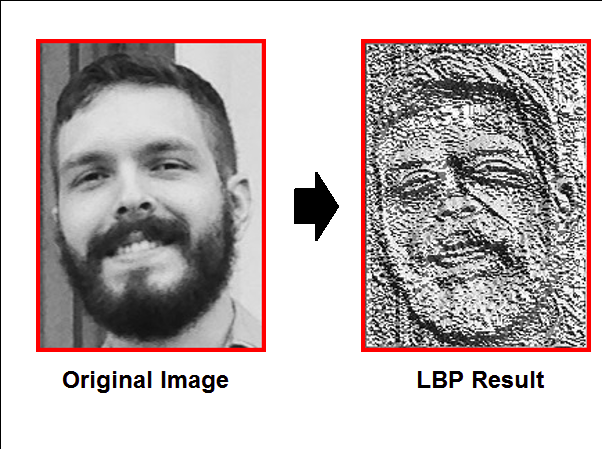
\includegraphics[scale=0.2]{img/lbp.png}
	%\caption{Diagram alur kerja}
	\caption{Local Binary Pattern}
	\label{fig: 3_27}
\end{figure}

\textit{Local Binary Pattern} (LBP) merupakan salah satu deskriptor visual yang digunakan pada visi komputer. Pada umumnya LBP digunakan pada Face Recognition dikarenakan LBP merupakan deskriptor yang sangat kuat untuk melakukan klasifikasi tekstur. Selain itu telah ditemukan bahwa ketika LBP digabungkan dengan deskriptor \textit{Histogram of Oriented Gradients} (HOG), performa yang didapatkan bertambah secara drastis pada beberapa dataset tertentu.

\par Cara kerja dari LBP sendiri adalah sebagai berikut:
\begin{enumerate}
	\vspace{-2mm}
	\item Ubah citra menjadi bentuk \textit{grayscale} / hitam putih.
	\vspace{-2mm}
	\item Bagi citra menjadi beberapa bagian(\textit{cell})
	\vspace{-2mm}
	\item Untuk setiap \textit{pixel} yang terdapat pada sebuah \textit{cell}, bandingkan dengan pixel milik 8 neighbor yang terdapat di sekelilingnya
	\vspace{-2mm}
	\item Apabila nilai dari pixel yang di tengah lebih besar dari setiap pixel pada neighbornya maka pixel tersebut diberi nilai 0, selain itu pixel tersebut diberi nilai 1.
	\vspace{-2mm}
	\item Hitung Histogram
	\vspace{-2mm}
	\item Normalisasi Histogram.
\end{enumerate}

\vspace{1ex}

\section{\textit{Fully-Connected Layer}}
\vspace{1ex}
\textit{Fully Connected layer} merupakan \textit{layer} yang bertujuan untuk melakukan transformasi pada dimensi data agar klasifikasi secara linear dapat dilakukan, dimana setiap neuron pada \textit{convolution layer} ditransformasi terlebih dahulu menjadi satu dimensi. Namun hal tersebut dapat menyebabkan hilangnya data spasial, sehingga pada umumnya fully connected layer hanya diimplementasikan pada akhir jaringan. \textit{Convolution layer} dengan ukuran kernel 1x1 dapat melakukan fungsi yang sama dengan \textit{Fully Connected Layer}, namun dapat tetap mempertahankan data spasial.
\vspace{1ex}

\section{\textit{Residual Network}}
\vspace{1ex}

\begin{figure}[h!]
	\centering
	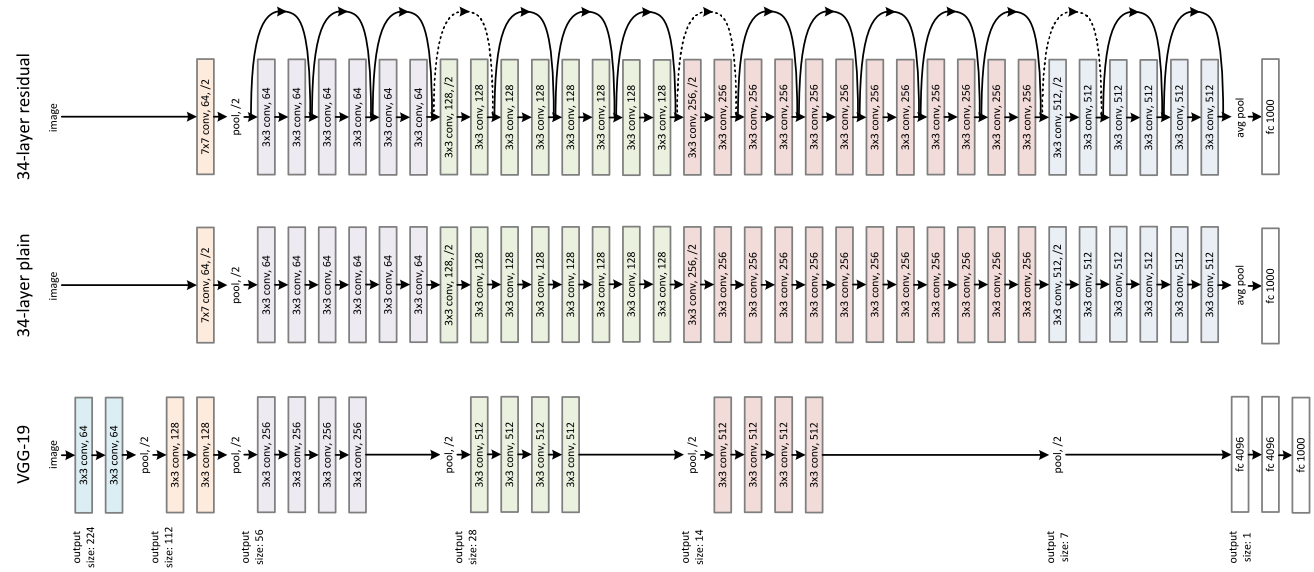
\includegraphics[scale=0.18]{img/ResNet.png}
	\caption{Perbandingan layer ResNet, plain, dan VGG-19 \cite{cit:10}}
	\label{fig:Resnet}
\end{figure}
\vspace{1ex}

\textit{Residual Neural Network} atau \textit{ResNet} merupakan sebuah \textit{Artificial Neural Network} (ANN) yang dibuat berdasarkan bentuk korteks serebral milik manusia. \textit{Residual Network} melakukan hal ini dengan memperkenalkan \textit{skip connection} atau \textit{shortcut}, dimana model dapat melompat dua atau tiga \textit{layer} jika memang hal tersebut merupakan hasil terbaik. Sebelum adanya model \textit{Residual Neural Network} penambahan layer pada suatu model hanya akan meningkatkan akurasi sampai suatu batas tertentu, sehingga penambahan layer setelah 20 hanya menambahkan kompleksitas model. Namun pada penelitian \textit{Deep Residual Learning for Image Recognition} yang dibuat oleh Kaiming He pada tahun 2015 memproposikan sebaliknya, apabila layer tambahan yang ada dapat mempelajari matriks identitas, maka akurasi minimal yang didapat pada \textit{layer} akan sama dengan apabila tidak menambahkan \textit{layer}. Untuk membuktikan hal tersebut dibuatlah sistem \textit{skip connection} atau \textit{shortcut} sehingga model dapat mempelajari matriks identitas dengan lebih mudah. Dari penelitian yang dilakukan pada dataset \textit{ImageNet}, \textit{Residual Network} dapat mengurangi \textit{loss} yang didapat ketika menambahkan lebih banyak \textit{layer} pada \textit{Artificial Neural Network} yang dibuat. \cite{cit:10}

\section{\textit{Lightweight Residual Network}}
\vspace{1ex}

\begin{figure}[h!]
	\centering
	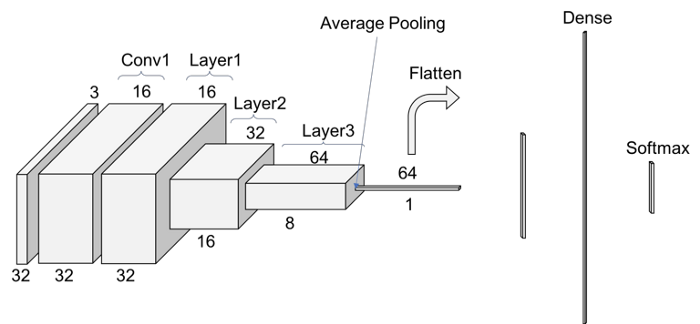
\includegraphics[scale=0.3]{img/StructureLightweightResNet.png}
	\caption{Skema struktur ResNet pada CIFAR10}
	\label{fig:ResnetScheme}
\end{figure}

Lightweight Residual Network merupakan implementasi dari Residual Network pada dataset CIFAR-10, sebuah dataset yang terdiri dari 60000 gambar 32x32, dimana setiap kelas memiliki 6000 gambar. Residual Network yang digunakan untuk memecahkan masalah klasifikasi CIFAR-10 ini berbeda dengan Residual Network pada normalnya yang memiliki jumlah parameter jauh lebih besar, yaitu sekitar 23 juta parameter. Residual Network ini memiliki jumlah layer yang relatif dalam apabila dibandingkan dengan Residual Network yang \textit{original}, namun parameter yang terdapat pada model ini jauh lebih sedikit, dengan yang paling banyak sebesar 3 juta parameter. Hal ini dikarenakan jumlah filter yang digunakan oleh model lightweight jauh lebih sedikit dibandingkan pada model konvensional, dimana pada model ResNet 50 filter yang digunakan adalah sebanyak 64 hingga 2048 filter, sedangkan pada model ResNet 56 filter yang digunakan hanyalah sebanyak 16 hingga 64 filter.

Pada gambar \ref{fig:ResnetScheme} dapat dilihat skema yang secara umum digunakan oleh Residual Network pada CIFAR10, dimana terlihat pada skema bahwa tidak terdapat \textit{pooling layer} setelah \textit{convolution layer}. Pada \textit{convolution layer} ini dapat dilihat bahwa layer pertama merupakan \textit{convolution layer} dengan ukuran 3x3 dan batch normalization. Ukuran \textit{stride} dan \textit{padding} yang diberikan adalah 1 untuk menyamakan bentuk output dengan input. Convolution Layer dari ResNet dapat dilihat dari gambar \ref{fig:Resnetconv}.

Kemudian setelah \textit{Convolution Layer}, dibuat sebuah layer yang terdiri dari 6 konvolusi dengan ukuran 3x3, banyaknya kumpulan konvolusi yang digunakan akan menentukan ukuran ResNet yang dibuat. Penurunan dimensi dari data dilakukan pada tahap ini dengan melakukan penambahan \textit{stride} menjadi dua untuk setiap konvolusi pertama di setiap layer berikut. 

\begin{figure}[h!]
	\centering
	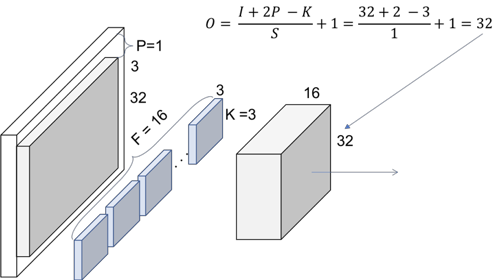
\includegraphics[scale=0.35]{img/convlightresnet.png}
	\caption{Convolution Layer Residual Network}
	\label{fig:Resnetconv}
\end{figure}

Pada layer ini diberikan \textit{bypass connection}, dimana apabila terjadi pengurangan performa dari model, dapat dilakukan \textit{bypass connection} dengan cara menambah padding dimensi dengan \textit{zeros} sehingga ukuran output sesuai dengan ukuran sebelumnya.

\begin{figure}[h!]
	\centering
	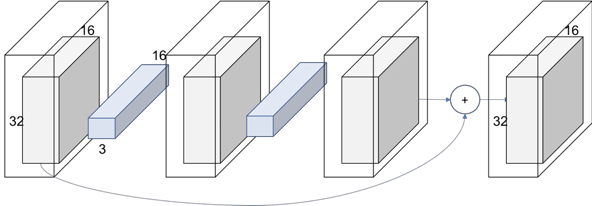
\includegraphics[scale=0.3]{img/layer1.png}
	\caption{Layer1 Residual Network}
	\label{fig:ResnetLayer1}
\end{figure}

Layer kedua memiliki cara kerja yang sama dengan layer pertama, namun dikarenakan ukuran \textit{stride} pada layer pertama dibuat menjadi dua, ukuran output adalah setengah dari input untuk layer kedua, sehingga diberikan \textit{zero padding}.

\begin{figure}[h!]
	\centering
	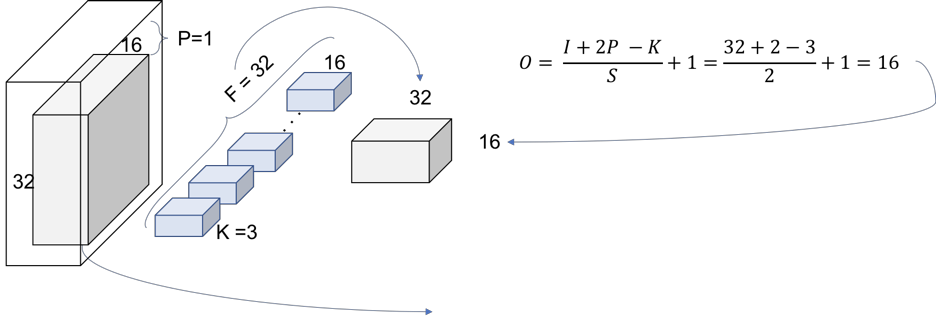
\includegraphics[scale=0.3]{img/layer2.png}
	\caption{Layer2 Residual Network}
	\label{fig:ResnetLayer2}
\end{figure}


Kemudian Layer 3 akan mengimplementasikan prinsip yang sama dengan Layer 2.

\begin{figure}[h!]
	\centering
	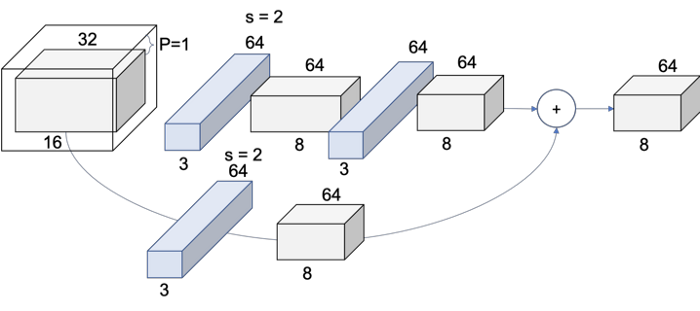
\includegraphics[scale=0.3]{img/layer3.png}
	\caption{Layer3 Residual Network}
	\label{fig:ResnetLayer3}
\end{figure}

\pagebreak

Sehingga formula akhir dari struktur Lightweight Residual Network dapat disimpulkan sebagai berikut \ref{fig:ResnetLayerFormula}

\begin{figure}[h!]
	\centering
	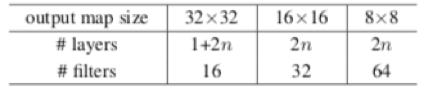
\includegraphics[scale=0.4]{img/ResNetFormula.png}
	\caption{Residual Network Formula}
	\label{fig:ResnetLayerFormula}
\end{figure}

Berikut merupakan perbandingan parameter Lightweight Residual Network dengan Residual Network

\begin{table}[h!]
	\begin{center}
		\begin{tabular}{|c|c|}
			\hline
			\textbf{Name} & \textbf{Parameters} \\ \hline
			ResNet 20 & 0.27M \\ \hline
			ResNet 32 & 0.46M \\ \hline
			ResNet 44 & 0.66M \\ \hline
			ResNet 56 & 0.85M \\ \hline
			ResNet 110 & 1.7M \\ \hline
			ResNet 50 & 23M \\ \hline
		\end{tabular}
	\end{center}
	\vspace{1ex}
	\caption{Parameter ResNet dibandingkan dengan Lightweight ResNet}
	\label{tabel:1}
\end{table}

\pagebreak

\section{Metode Pengujian}
\vspace{1ex}

\subsection{\textit{Precision}}
\vspace{1ex}
\textit{Precision} merupakan rasio dari prediksi jumlah total contoh positif yang benar diklasifikasikan dibagi dengan jumlah keseluruhan hasil yang diprediksi positif. Precision dapat melihat dari keseluruhan data, berapa persen yang diklasifikasikan secara benar.
\[Recall = \frac{TP}{(TP+FP)}\]

\subsection{\textit{Recall}}
\vspace{1ex}
Recall merupakan rasio dari jumlah total positif yang benar diklasifikasikan, dibagi dengan jumlah total contoh yang benar positif. Recall yang tinggi menunjukan bahwa kelas yang dikenali dengan benar banyak, atau False Negative yang didapatkan sedikit.
\[Recall = \frac{TP}{(TP+FN)}\]

\subsection{\textit{mean Average Precision} (mAP)}
\vspace{1ex}
\textit{mean Average Precision} (mAP) merupakan sebuah metrik akurasi yang didapatkan dari rata rata \textit{Average Precision}. Dimana Average Precision sendiri didapatkan dari perhitungan nilai presisi dan recall. mean Average Precision merupakan sebuah metrik evaluasi yang sangat baik dikarenakan melibatkan presisi dan recall. Dengan menggunakan mean Average Precision, sebuah angka dapat diterima untuk mengukur kinerja dari pendeteksian sebuah objek.

\[AP = \Sigma (recall_{n+1})-recall_n)\times precision_{interp}\times(recall_{n+1})\]

\subsection{\textit{Precision at n}}
\vspace{1ex}
\textit{Precision at n} merupakan sebuah metrik evaluasi yang didapatkan dari pengembalian informasi dalam bentuk daftar dengan ranking. Daftar ranking tersebut kemudian digunakan untuk melakukan penilaian dari akurasi model dengan cara melihat informasi ke-n paling atas yang dikembalikan. Rank-1 accuracy merupakan pengecekan berapa kali prediksi label sesuai dengan yang sebenarnya, sedangkan Rank-5 accuracy merupakan berapa kali prediksi label terdapat pada 5 prediksi paling atas.

\subsection{\textit{Re-Ranking}}
\vspace{1ex}
\textit{Re-Ranking} merupakan pengambilan \textit{K-Recriprocal Nearest Neighbor} yang mengambil citra serupa dengan citra \textit{query} yang diberikan. Hal ini dilakukan dengan adanya pengambilan jarak antara citra \textit{query} dengan citra yang terdapat pada \textit{gallery}.
  \cleardoublepage

  % Bab 3 desain dan implementasi
  \chapter{DATA DAN METODOLOGI}
\vspace{1ex}

\section*{}
Penelitian ini dilaksanakan sesuai dengan desain sistem berikut dengan implementasinya. Desain sistem merupakan konsep dari pembuatan dan perancangan infrastruktur kemudian diwujudkan dalam bentuk blok-blok alur yang harus dikerjakan. Pada bagian implementasi merupakan pelaksanaan teknis untuk setiap blok pada desain sistem.
\vspace{1ex}

\section{Cakupan Tugas Akhir}
\vspace{1ex}

Tugas akhir ini merupakan salah satu bentuk implementasi Lightweight Convolutional Neural Network untuk melakukan pencarian seorang individu menggunakan gambar multi-modal berupa sketsa sebagai input, berikut pada Gambar 3.1 adalah cakupan Tugas Akhir dari Desain Sistem.
\begin{figure}  [!htb]
	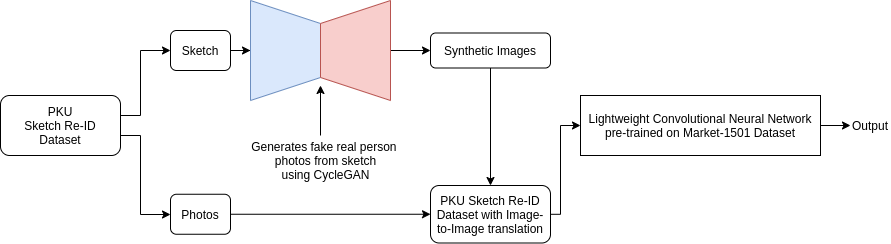
\includegraphics[scale=0.35]{img/desain_sistem.png}
	\caption{Desain Sistem}
	\label{fig: 3_1}
\end{figure}
\vspace{1ex}

\section{Penyesuaian Dataset PKU Sketch Re-ID}
Desain sistem secara umum pada gambar \ref{fig: 3_1}, yang mencakup beberapa hal, salah satunya ialah penyesuaian dataset. Dataset yang kami akan gunakan adalah dataset PKU Sketch Re-ID yang dibuat oleh Lu Pang \cite{cit:15}. Dataset ini terdiri dari 200 identitas yang unik, dimana setiap identitas telah ditangkap oleh dua kamera berbeda. Selain itu setiap individu memiliki satu gambar sketsa, sehingga seluruh dataset bertotal 600 gambar. Gambar \ref{fig: 3_2} menunjukkan beberapa contoh dari dataset PKU Sketch Re-ID. 

\begin{figure}  [!htb]
	\centering
	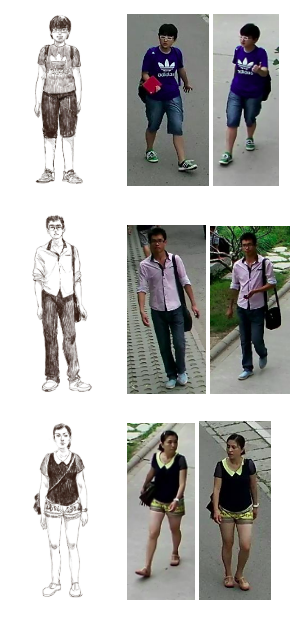
\includegraphics[scale=0.35]{img/ExamplesSketchReID.png}
	\caption{Beberapa contoh gambar pada Dataset PKU Sketch Re-ID}
	\label{fig: 3_2}
\end{figure}

Dataset PKU Sketch \cite{cit:15} Re-id kemudian akan melalui proses persiapan terlebih dahulu sehingga dapat dilakukan evaluasi performa dari Lightweight Convolutional Neural Network yang akan digunakan. Penyesuaian yang akan dilakukan pada dataset meliputi, penggabungan individu-individu sama yang tertangkap oleh kamera kamera berbeda, kemudian pemasangan individu tersebut ke gambar sketsa sehingga setiap individu unik akan menjadi kelas tersendiri. Kemudian dataset tersebut akan dibagi menjadi 150 identitas untuk training dan 50 identitas untuk testing, seperti yang ditunjukan pada gambar \ref{fig: 3_3}. Setiap gambar telah di \textit{crop} secara \textit{manual} untuk memastikan setiap gambar dari dataset hanya berisi satu individu yang spesifik. Untuk gambar sketsa yang digunakan, terdapat 5 orang seniman berbeda yang memiliki 5 \textit{art style} yang berbeda pula untuk menggambar masing masing identitas. 

\begin{figure}  [!htb]
	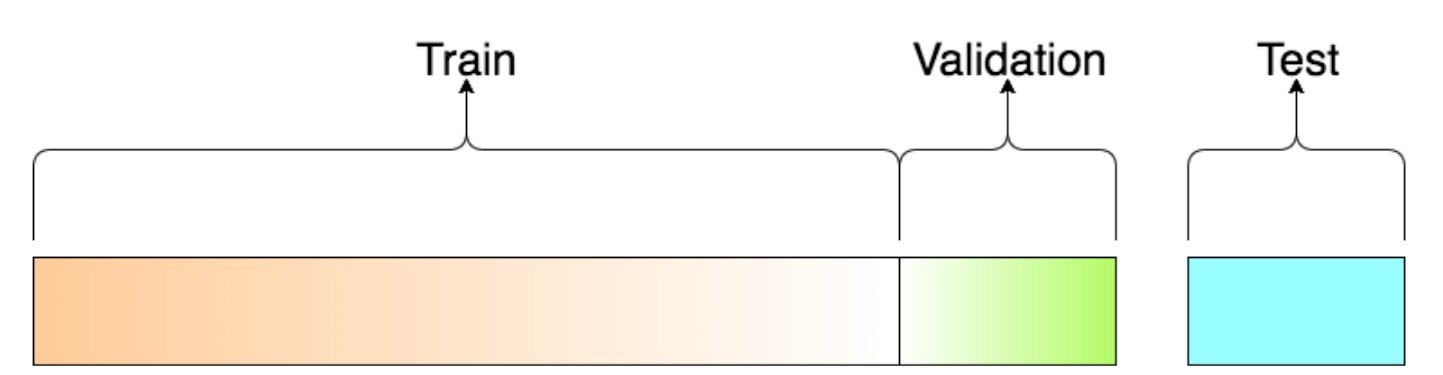
\includegraphics[scale=0.35]{img/dataset.png}
	\caption{Pembagian Dataset PKU Sketch Re-ID}
	\label{fig: 3_3}
\end{figure}

\section{Lightweight Convolutional Neural Network}
Setelah penyesuaian dataset telah dilakukan, akan dilakukan training dengan menggunakan Lightweight Residual Network yang pernah digunakan untuk memecahkan masalah klasifikasi CIFAR-10. Namun pada model yang kami gunakan, \textit{Fully-Connected Layer} terakhir dihilangkan, dan ditambahkan dua layer baru untuk menggantikan layer tersebut sehingga model dapat dipastikan akan mempelajari fitur-fitur yang terdapat pada dataset PKU Sketch Re-ID. Digunakan dua buah Fully-Connected layer supaya pada Fully Connected layer pertama dapat dilakukan pengenalan fitur diskriminan dari masing-masing individu, dan pada layer kedua dilakukan klasifikasi dari masing-masing individu tersebut. Selain itu, berbeda dengan model ResNet aslinya, model yang kami gunakan menggunakan resolusi input sebesar 32x64x3.

\begin{table}[h!]
	\begin{center}
		\begin{tabular}{|c|c|}
			\hline
			\textbf{Nama} & \textbf{Parameter} \\ \hline
			ResNet 56 & 0.85M \\ \hline
			ResNet 110 & 1.7M \\ \hline
			GoogleNet & 7M \\ \hline
			DenseNet121 & 8.6M \\ \hline
			ResNet 50 & 23M \\ \hline
		\end{tabular}
	\end{center}
	\vspace{1ex}
	\caption{Jumlah parameter untuk beberapa model popular.}
	\label{tabel:2}
\end{table}

Pada percobaan-percobaan yang kami lakukan, kami menggunakan tiga model Residual Network yang berbeda, yaitu ResNet 20, ResNet 56, dan ResNet 110. Namun kami hanya melanjutkan menggunakan ResNet 56 dan ResNet 110 dikarenakan kedua model tersebut mendapatkan hasil yang jauh lebih baik dibandingkan dengan pada ResNet 20. Meskipun layer dari kedua model yang kami gunakan relatif cukup dalam (56 dan 110 layer) apabila dibandingkan dengan Residual Network normalnya. Parameter yang terdapat pada model ini jauh lebih sedikit, dimana ResNet 110 hanya memiliki 1.7 juta parameter, jauh dari jutaan parameter yang dimiliki model-model populer seperti DenseNet, GoogleNet, dan ResNet 50.Pada tabel \ref{tab:long} dapat dilihat bentuk susunan layer dari ResNet 20 sendiri. Untuk susunan model ResNet 56 dapat dilihat pada \ref{tab:long2} dan untuk ResNet 110 dapat dilihat pada \ref{tab:long3}.

\begin{center}
	\begin{longtable}{|l|l|l|l|}
		\caption{Susunan Model ResNet 20} \label{tab:long} \\
		
		\hline \multicolumn{1}{|c|}{\textbf{Type}} & \multicolumn{1}{c|}{\textbf{Channel}} & \multicolumn{1}{c|}{\textbf{Size}} & \multicolumn{1}{c|}{\textbf{Stride}}\\ \hline 
		\endfirsthead
		
		\multicolumn{4}{c}%
		{{\bfseries \tablename\ \thetable{} -- Dilanjutkan dari halaman sebelumnya}} \\
		\hline \multicolumn{1}{|c|}{\textbf{Type}} & \multicolumn{1}{c|}{\textbf{Channel}} & \multicolumn{1}{c|}{\textbf{Size}} & \multicolumn{1}{c|}{\textbf{Stride}}\\ \hline 
		\endhead
		
		\hline \multicolumn{4}{|r|}{{Dilanjutkan ke halaman selanjutnya}} \\ \hline
		\endfoot
		
		\hline \hline
		\endlastfoot
		Convolutional2D & 16 & 3x3 & 1x1 \\
		BatchNorm2D & 16 & \_ & \_ \\ 
		Convolutional2D & 16 & 3x3 & 1x1 \\
		BatchNorm2D & 16 & \_ & \_ \\
		Convolutional2D & 16 & 3x3 & 1x1 \\
		BatchNorm2D & 16 & \_ & \_ \\
		Convolutional2D & 16 & 3x3 & 1x1 \\
		BatchNorm2D & 16 & \_ & \_ \\
		Convolutional2D & 16 & 3x3 & 1x1 \\
		BatchNorm2D & 16 & \_ & \_ \\
		Convolutional2D & 16 & 3x3 & 1x1 \\
		BatchNorm2D & 16 & \_ & \_ \\
		Convolutional2D & 16 & 3x3 & 1x1 \\
		BatchNorm2D & 16 & \_ & \_ \\
		Convolutional2D & 32 & 3x3 & 2x2 \\
		BatchNorm2D & 32 & \_ & \_ \\
		Convolutional2D & 32 & 3x3 & 1x1 \\
		BatchNorm2D & 32 & \_ & \_ \\
		Convolutional2D & 32 & 3x3 & 1x1 \\
		BatchNorm2D & 32 & \_ & \_ \\
		Convolutional2D & 32 & 3x3 & 1x1 \\
		BatchNorm2D & 32 & \_ & \_ \\
		Convolutional2D & 32 & 3x3 & 1x1 \\
		BatchNorm2D & 32 & \_ & \_ \\
		Convolutional2D & 32 & 3x3 & 1x1 \\
		BatchNorm2D & 32 & \_ & \_ \\
		Convolutional2D & 64 & 3x3 & 2x2 \\
		BatchNorm2D & 64 & \_ & \_ \\
		Convolutional2D & 64 & 3x3 & 1x1 \\
		BatchNorm2D & 64 & \_ & \_ \\
		Convolutional2D & 64 & 3x3 & 1x1 \\
		BatchNorm2D & 64 & \_ & \_ \\
		Convolutional2D & 64 & 3x3 & 1x1 \\
		BatchNorm2D & 64 & \_ & \_ \\
		Convolutional2D & 64 & 3x3 & 1x1 \\
		BatchNorm2D & 64 & \_ & \_ \\
		Convolutional2D & 64 & 3x3 & 1x1 \\
		BatchNorm2D & 64 & \_ & \_ \\
		FullyConnected & \_ & \_ & \_ \\
		BatchNorm1D & 512 & \_ & \_ \\
		Dropout & \_ & \_ & \_ \\
		FullyConnected & \_ & \_ & \_ \\
	\end{longtable}
\end{center}

\begin{center}
	\begin{longtable}{|l|l|l|l|}
		\caption{Susunan Model ResNet 56} \label{tab:long2} \\
		
		\hline \multicolumn{1}{|c|}{\textbf{Type}} & \multicolumn{1}{c|}{\textbf{Channel}} & \multicolumn{1}{c|}{\textbf{Size}} & \multicolumn{1}{c|}{\textbf{Stride}}\\ \hline 
		\endfirsthead
		
		\multicolumn{4}{c}%
		{{\bfseries \tablename\ \thetable{} -- Dilanjutkan dari halaman sebelumnya}} \\
		\hline \multicolumn{1}{|c|}{\textbf{Type}} & \multicolumn{1}{c|}{\textbf{Channel}} & \multicolumn{1}{c|}{\textbf{Size}} & \multicolumn{1}{c|}{\textbf{Stride}}\\ \hline 
		\endhead
		
		\hline \multicolumn{4}{|r|}{{Dilanjutkan ke halaman selanjutnya}} \\ \hline
		\endfoot
		
		\hline \hline
		\endlastfoot
		Convolutional2D & 16 & 3x3 & 1x1 \\
		BatchNorm2D & 16 & \_ & \_ \\ 
		Convolutional2D & 16 & 3x3 & 1x1 \\
		BatchNorm2D & 16 & \_ & \_ \\
		Convolutional2D & 16 & 3x3 & 1x1 \\
		BatchNorm2D & 16 & \_ & \_ \\
		Convolutional2D & 16 & 3x3 & 1x1 \\
		BatchNorm2D & 16 & \_ & \_ \\
		Convolutional2D & 16 & 3x3 & 1x1 \\
		BatchNorm2D & 16 & \_ & \_ \\
		Convolutional2D & 16 & 3x3 & 1x1 \\
		BatchNorm2D & 16 & \_ & \_ \\
		Convolutional2D & 16 & 3x3 & 1x1 \\
		BatchNorm2D & 16 & \_ & \_ \\
		Convolutional2D & 16 & 3x3 & 1x1 \\
		BatchNorm2D & 16 & \_ & \_ \\
		Convolutional2D & 16 & 3x3 & 1x1 \\
		BatchNorm2D & 16 & \_ & \_ \\
		Convolutional2D & 16 & 3x3 & 1x1 \\
		BatchNorm2D & 16 & \_ & \_ \\
		Convolutional2D & 16 & 3x3 & 1x1 \\
		BatchNorm2D & 16 & \_ & \_ \\
		Convolutional2D & 16 & 3x3 & 1x1 \\
		BatchNorm2D & 16 & \_ & \_ \\
		Convolutional2D & 16 & 3x3 & 1x1 \\
		BatchNorm2D & 16 & \_ & \_ \\
		Convolutional2D & 16 & 3x3 & 1x1 \\
		BatchNorm2D & 16 & \_ & \_ \\
		Convolutional2D & 16 & 3x3 & 1x1 \\
		BatchNorm2D & 16 & \_ & \_ \\
		Convolutional2D & 16 & 3x3 & 1x1 \\
		BatchNorm2D & 16 & \_ & \_ \\
		Convolutional2D & 16 & 3x3 & 1x1 \\
		BatchNorm2D & 16 & \_ & \_ \\
		Convolutional2D & 16 & 3x3 & 1x1 \\
		BatchNorm2D & 16 & \_ & \_ \\
		Convolutional2D & 16 & 3x3 & 1x1 \\
		BatchNorm2D & 16 & \_ & \_ \\
		Convolutional2D & 32 & 3x3 & 2x2 \\
		BatchNorm2D & 32 & \_ & \_ \\
		Convolutional2D & 32 & 3x3 & 1x1 \\
		BatchNorm2D & 32 & \_ & \_ \\
		Convolutional2D & 32 & 3x3 & 1x1 \\
		BatchNorm2D & 32 & \_ & \_ \\
		Convolutional2D & 32 & 3x3 & 1x1 \\
		BatchNorm2D & 32 & \_ & \_ \\
		Convolutional2D & 32 & 3x3 & 1x1 \\
		BatchNorm2D & 32 & \_ & \_ \\
		Convolutional2D & 32 & 3x3 & 1x1 \\
		BatchNorm2D & 32 & \_ & \_ \\
		Convolutional2D & 32 & 3x3 & 1x1 \\
		BatchNorm2D & 32 & \_ & \_ \\
		Convolutional2D & 32 & 3x3 & 1x1 \\
		BatchNorm2D & 32 & \_ & \_ \\
		Convolutional2D & 32 & 3x3 & 1x1 \\
		BatchNorm2D & 32 & \_ & \_ \\
		Convolutional2D & 32 & 3x3 & 1x1 \\
		BatchNorm2D & 32 & \_ & \_ \\
		Convolutional2D & 32 & 3x3 & 1x1 \\
		BatchNorm2D & 32 & \_ & \_ \\
		Convolutional2D & 32 & 3x3 & 1x1 \\
		BatchNorm2D & 32 & \_ & \_ \\
		Convolutional2D & 32 & 3x3 & 1x1 \\
		BatchNorm2D & 32 & \_ & \_ \\
		Convolutional2D & 32 & 3x3 & 1x1 \\
		BatchNorm2D & 32 & \_ & \_ \\
		Convolutional2D & 32 & 3x3 & 1x1 \\
		BatchNorm2D & 32 & \_ & \_ \\
		Convolutional2D & 32 & 3x3 & 1x1 \\
		BatchNorm2D & 32 & \_ & \_ \\
		Convolutional2D & 32 & 3x3 & 1x1 \\
		BatchNorm2D & 32 & \_ & \_ \\
		Convolutional2D & 32 & 3x3 & 1x1 \\
		BatchNorm2D & 32 & \_ & \_ \\
		Convolutional2D & 64 & 3x3 & 2x2 \\
		BatchNorm2D & 64 & \_ & \_ \\
		Convolutional2D & 64 & 3x3 & 1x1 \\
		BatchNorm2D & 64 & \_ & \_ \\
		Convolutional2D & 64 & 3x3 & 1x1 \\
		BatchNorm2D & 64 & \_ & \_ \\
		Convolutional2D & 64 & 3x3 & 1x1 \\
		BatchNorm2D & 64 & \_ & \_ \\
		Convolutional2D & 64 & 3x3 & 1x1 \\
		BatchNorm2D & 64 & \_ & \_ \\
		Convolutional2D & 64 & 3x3 & 1x1 \\
		BatchNorm2D & 64 & \_ & \_ \\
		Convolutional2D & 64 & 3x3 & 1x1 \\
		BatchNorm2D & 64 & \_ & \_ \\
		Convolutional2D & 64 & 3x3 & 1x1 \\
		BatchNorm2D & 64 & \_ & \_ \\
		Convolutional2D & 64 & 3x3 & 1x1 \\
		BatchNorm2D & 64 & \_ & \_ \\
		Convolutional2D & 64 & 3x3 & 1x1 \\
		BatchNorm2D & 64 & \_ & \_ \\
		Convolutional2D & 64 & 3x3 & 1x1 \\
		BatchNorm2D & 64 & \_ & \_ \\
		Convolutional2D & 64 & 3x3 & 1x1 \\
		BatchNorm2D & 64 & \_ & \_ \\
		Convolutional2D & 64 & 3x3 & 1x1 \\
		BatchNorm2D & 64 & \_ & \_ \\
		Convolutional2D & 64 & 3x3 & 1x1 \\
		BatchNorm2D & 64 & \_ & \_ \\
		Convolutional2D & 64 & 3x3 & 1x1 \\
		BatchNorm2D & 64 & \_ & \_ \\
		Convolutional2D & 64 & 3x3 & 1x1 \\
		BatchNorm2D & 64 & \_ & \_ \\
		Convolutional2D & 64 & 3x3 & 1x1 \\
		BatchNorm2D & 64 & \_ & \_ \\
		Convolutional2D & 64 & 3x3 & 1x1 \\
		BatchNorm2D & 64 & \_ & \_ \\
		FullyConnected & \_ & \_ & \_ \\
		BatchNorm1D & 512 & \_ & \_ \\
		Dropout & \_ & \_ & \_ \\
		FullyConnected & \_ & \_ & \_ \\
	\end{longtable}
\end{center}

\begin{center}
	\begin{longtable}{|l|l|l|l|}
		\caption{Susunan Model ResNet 110} \label{tab:long3} \\
		
		\hline \multicolumn{1}{|c|}{\textbf{Type}} & \multicolumn{1}{c|}{\textbf{Channel}} & \multicolumn{1}{c|}{\textbf{Size}} & \multicolumn{1}{c|}{\textbf{Stride}}\\ \hline 
		\endfirsthead
		
		\multicolumn{4}{c}%
		{{\bfseries \tablename\ \thetable{} -- Dilanjutkan dari halaman sebelumnya}} \\
		\hline \multicolumn{1}{|c|}{\textbf{Type}} & \multicolumn{1}{c|}{\textbf{Channel}} & \multicolumn{1}{c|}{\textbf{Size}} & \multicolumn{1}{c|}{\textbf{Stride}}\\ \hline 
		\endhead
		
		\hline \multicolumn{4}{|r|}{{Dilanjutkan ke halaman selanjutnya}} \\ \hline
		\endfoot
		
		\hline \hline
		\endlastfoot
		Convolutional2D & 16 & 3x3 & 1x1 \\
		BatchNorm2D & 16 & \_ & \_ \\ 
		Convolutional2D & 16 & 3x3 & 1x1 \\
		BatchNorm2D & 16 & \_ & \_ \\
		Convolutional2D & 16 & 3x3 & 1x1 \\
		BatchNorm2D & 16 & \_ & \_ \\
		Convolutional2D & 16 & 3x3 & 1x1 \\
		BatchNorm2D & 16 & \_ & \_ \\
		Convolutional2D & 16 & 3x3 & 1x1 \\
		BatchNorm2D & 16 & \_ & \_ \\
		Convolutional2D & 16 & 3x3 & 1x1 \\
		BatchNorm2D & 16 & \_ & \_ \\
		Convolutional2D & 16 & 3x3 & 1x1 \\
		BatchNorm2D & 16 & \_ & \_ \\
		Convolutional2D & 16 & 3x3 & 1x1 \\
		BatchNorm2D & 16 & \_ & \_ \\
		Convolutional2D & 16 & 3x3 & 1x1 \\
		BatchNorm2D & 16 & \_ & \_ \\
		Convolutional2D & 16 & 3x3 & 1x1 \\
		BatchNorm2D & 16 & \_ & \_ \\
		Convolutional2D & 16 & 3x3 & 1x1 \\
		BatchNorm2D & 16 & \_ & \_ \\
		Convolutional2D & 16 & 3x3 & 1x1 \\
		BatchNorm2D & 16 & \_ & \_ \\
		Convolutional2D & 16 & 3x3 & 1x1 \\
		BatchNorm2D & 16 & \_ & \_ \\
		Convolutional2D & 16 & 3x3 & 1x1 \\
		BatchNorm2D & 16 & \_ & \_ \\
		Convolutional2D & 16 & 3x3 & 1x1 \\
		BatchNorm2D & 16 & \_ & \_ \\
		Convolutional2D & 16 & 3x3 & 1x1 \\
		BatchNorm2D & 16 & \_ & \_ \\
		Convolutional2D & 16 & 3x3 & 1x1 \\
		BatchNorm2D & 16 & \_ & \_ \\
		Convolutional2D & 16 & 3x3 & 1x1 \\
		BatchNorm2D & 16 & \_ & \_ \\
		Convolutional2D & 16 & 3x3 & 1x1 \\
		BatchNorm2D & 16 & \_ & \_ \\
		Convolutional2D & 16 & 3x3 & 1x1 \\
		BatchNorm2D & 16 & \_ & \_ \\
		Convolutional2D & 16 & 3x3 & 1x1 \\
		BatchNorm2D & 16 & \_ & \_ \\
		Convolutional2D & 16 & 3x3 & 1x1 \\
		BatchNorm2D & 16 & \_ & \_ \\
		Convolutional2D & 16 & 3x3 & 1x1 \\
		BatchNorm2D & 16 & \_ & \_ \\
		Convolutional2D & 16 & 3x3 & 1x1 \\
		BatchNorm2D & 16 & \_ & \_ \\
		Convolutional2D & 16 & 3x3 & 1x1 \\
		BatchNorm2D & 16 & \_ & \_ \\
		Convolutional2D & 16 & 3x3 & 1x1 \\
		BatchNorm2D & 16 & \_ & \_ \\
		Convolutional2D & 16 & 3x3 & 1x1 \\
		BatchNorm2D & 16 & \_ & \_ \\
		Convolutional2D & 16 & 3x3 & 1x1 \\
		BatchNorm2D & 16 & \_ & \_ \\
		Convolutional2D & 16 & 3x3 & 1x1 \\
		BatchNorm2D & 16 & \_ & \_ \\
		Convolutional2D & 16 & 3x3 & 1x1 \\
		BatchNorm2D & 16 & \_ & \_ \\
		Convolutional2D & 16 & 3x3 & 1x1 \\
		BatchNorm2D & 16 & \_ & \_ \\
		Convolutional2D & 16 & 3x3 & 1x1 \\
		BatchNorm2D & 16 & \_ & \_ \\
		Convolutional2D & 16 & 3x3 & 1x1 \\
		BatchNorm2D & 16 & \_ & \_ \\
		Convolutional2D & 16 & 3x3 & 1x1 \\
		BatchNorm2D & 16 & \_ & \_ \\
		Convolutional2D & 16 & 3x3 & 1x1 \\
		BatchNorm2D & 16 & \_ & \_ \\
		Convolutional2D & 16 & 3x3 & 1x1 \\
		BatchNorm2D & 16 & \_ & \_ \\
		Convolutional2D & 16 & 3x3 & 1x1 \\
		BatchNorm2D & 16 & \_ & \_ \\
		Convolutional2D & 32 & 3x3 & 2x2 \\
		BatchNorm2D & 32 & \_ & \_ \\
		Convolutional2D & 32 & 3x3 & 1x1 \\
		BatchNorm2D & 32 & \_ & \_ \\
		Convolutional2D & 32 & 3x3 & 1x1 \\
		BatchNorm2D & 32 & \_ & \_ \\
		Convolutional2D & 32 & 3x3 & 1x1 \\
		BatchNorm2D & 32 & \_ & \_ \\
		Convolutional2D & 32 & 3x3 & 1x1 \\
		BatchNorm2D & 32 & \_ & \_ \\
		Convolutional2D & 32 & 3x3 & 1x1 \\
		BatchNorm2D & 32 & \_ & \_ \\
		Convolutional2D & 32 & 3x3 & 1x1 \\
		BatchNorm2D & 32 & \_ & \_ \\
		Convolutional2D & 32 & 3x3 & 1x1 \\
		BatchNorm2D & 32 & \_ & \_ \\
		Convolutional2D & 32 & 3x3 & 1x1 \\
		BatchNorm2D & 32 & \_ & \_ \\
		Convolutional2D & 32 & 3x3 & 1x1 \\
		BatchNorm2D & 32 & \_ & \_ \\
		Convolutional2D & 32 & 3x3 & 1x1 \\
		BatchNorm2D & 32 & \_ & \_ \\
		Convolutional2D & 32 & 3x3 & 1x1 \\
		BatchNorm2D & 32 & \_ & \_ \\
		Convolutional2D & 32 & 3x3 & 1x1 \\
		BatchNorm2D & 32 & \_ & \_ \\
		Convolutional2D & 32 & 3x3 & 1x1 \\
		BatchNorm2D & 32 & \_ & \_ \\
		Convolutional2D & 32 & 3x3 & 1x1 \\
		BatchNorm2D & 32 & \_ & \_ \\
		Convolutional2D & 32 & 3x3 & 1x1 \\
		BatchNorm2D & 32 & \_ & \_ \\
		Convolutional2D & 32 & 3x3 & 1x1 \\
		BatchNorm2D & 32 & \_ & \_ \\
		Convolutional2D & 32 & 3x3 & 1x1 \\
		BatchNorm2D & 32 & \_ & \_ \\
		Convolutional2D & 32 & 3x3 & 1x1 \\
		BatchNorm2D & 32 & \_ & \_ \\
		Convolutional2D & 32 & 3x3 & 1x1 \\
		BatchNorm2D & 32 & \_ & \_ \\
		Convolutional2D & 32 & 3x3 & 1x1 \\
		BatchNorm2D & 32 & \_ & \_ \\
		Convolutional2D & 32 & 3x3 & 1x1 \\
		BatchNorm2D & 32 & \_ & \_ \\
		Convolutional2D & 32 & 3x3 & 1x1 \\
		BatchNorm2D & 32 & \_ & \_ \\
		Convolutional2D & 32 & 3x3 & 1x1 \\
		BatchNorm2D & 32 & \_ & \_ \\
		Convolutional2D & 32 & 3x3 & 1x1 \\
		BatchNorm2D & 32 & \_ & \_ \\
		Convolutional2D & 32 & 3x3 & 1x1 \\
		BatchNorm2D & 32 & \_ & \_ \\
		Convolutional2D & 32 & 3x3 & 1x1 \\
		BatchNorm2D & 32 & \_ & \_ \\
		Convolutional2D & 32 & 3x3 & 1x1 \\
		BatchNorm2D & 32 & \_ & \_ \\
		Convolutional2D & 32 & 3x3 & 1x1 \\
		BatchNorm2D & 32 & \_ & \_ \\
		Convolutional2D & 32 & 3x3 & 1x1 \\
		BatchNorm2D & 32 & \_ & \_ \\
		Convolutional2D & 32 & 3x3 & 1x1 \\
		BatchNorm2D & 32 & \_ & \_ \\
		Convolutional2D & 32 & 3x3 & 1x1 \\
		BatchNorm2D & 32 & \_ & \_ \\
		Convolutional2D & 32 & 3x3 & 1x1 \\
		BatchNorm2D & 32 & \_ & \_ \\
		Convolutional2D & 32 & 3x3 & 1x1 \\
		BatchNorm2D & 32 & \_ & \_ \\
		Convolutional2D & 32 & 3x3 & 1x1 \\
		BatchNorm2D & 32 & \_ & \_ \\
		Convolutional2D & 32 & 3x3 & 1x1 \\
		BatchNorm2D & 32 & \_ & \_ \\
		Convolutional2D & 64 & 3x3 & 2x2 \\
		BatchNorm2D & 64 & \_ & \_ \\
		Convolutional2D & 64 & 3x3 & 1x1 \\
		BatchNorm2D & 64 & \_ & \_ \\
		Convolutional2D & 64 & 3x3 & 1x1 \\
		BatchNorm2D & 64 & \_ & \_ \\
		Convolutional2D & 64 & 3x3 & 1x1 \\
		BatchNorm2D & 64 & \_ & \_ \\
		Convolutional2D & 64 & 3x3 & 1x1 \\
		BatchNorm2D & 64 & \_ & \_ \\
		Convolutional2D & 64 & 3x3 & 1x1 \\
		BatchNorm2D & 64 & \_ & \_ \\
		Convolutional2D & 64 & 3x3 & 1x1 \\
		BatchNorm2D & 64 & \_ & \_ \\
		Convolutional2D & 64 & 3x3 & 1x1 \\
		BatchNorm2D & 64 & \_ & \_ \\
		Convolutional2D & 64 & 3x3 & 1x1 \\
		BatchNorm2D & 64 & \_ & \_ \\
		Convolutional2D & 64 & 3x3 & 1x1 \\
		BatchNorm2D & 64 & \_ & \_ \\
		Convolutional2D & 64 & 3x3 & 1x1 \\
		BatchNorm2D & 64 & \_ & \_ \\
		Convolutional2D & 64 & 3x3 & 1x1 \\
		BatchNorm2D & 64 & \_ & \_ \\
		Convolutional2D & 64 & 3x3 & 1x1 \\
		BatchNorm2D & 64 & \_ & \_ \\
		Convolutional2D & 64 & 3x3 & 1x1 \\
		BatchNorm2D & 64 & \_ & \_ \\
		Convolutional2D & 64 & 3x3 & 1x1 \\
		BatchNorm2D & 64 & \_ & \_ \\
		Convolutional2D & 64 & 3x3 & 1x1 \\
		BatchNorm2D & 64 & \_ & \_ \\
		Convolutional2D & 64 & 3x3 & 1x1 \\
		BatchNorm2D & 64 & \_ & \_ \\
		Convolutional2D & 64 & 3x3 & 1x1 \\
		BatchNorm2D & 64 & \_ & \_ \\
		Convolutional2D & 64 & 3x3 & 1x1 \\
		BatchNorm2D & 64 & \_ & \_ \\
		Convolutional2D & 64 & 3x3 & 1x1 \\
		BatchNorm2D & 64 & \_ & \_ \\
		Convolutional2D & 64 & 3x3 & 1x1 \\
		BatchNorm2D & 64 & \_ & \_ \\
		Convolutional2D & 64 & 3x3 & 1x1 \\
		BatchNorm2D & 64 & \_ & \_ \\
		Convolutional2D & 64 & 3x3 & 1x1 \\
		BatchNorm2D & 64 & \_ & \_ \\
		Convolutional2D & 64 & 3x3 & 1x1 \\
		BatchNorm2D & 64 & \_ & \_ \\
		Convolutional2D & 64 & 3x3 & 1x1 \\
		BatchNorm2D & 64 & \_ & \_ \\
		Convolutional2D & 64 & 3x3 & 1x1 \\
		BatchNorm2D & 64 & \_ & \_ \\
		Convolutional2D & 64 & 3x3 & 1x1 \\
		BatchNorm2D & 64 & \_ & \_ \\
		Convolutional2D & 64 & 3x3 & 1x1 \\
		BatchNorm2D & 64 & \_ & \_ \\
		Convolutional2D & 64 & 3x3 & 1x1 \\
		BatchNorm2D & 64 & \_ & \_ \\
		Convolutional2D & 64 & 3x3 & 1x1 \\
		BatchNorm2D & 64 & \_ & \_ \\
		Convolutional2D & 64 & 3x3 & 1x1 \\
		BatchNorm2D & 64 & \_ & \_ \\
		Convolutional2D & 64 & 3x3 & 1x1 \\
		BatchNorm2D & 64 & \_ & \_ \\
		Convolutional2D & 64 & 3x3 & 1x1 \\
		BatchNorm2D & 64 & \_ & \_ \\
		Convolutional2D & 64 & 3x3 & 1x1 \\
		BatchNorm2D & 64 & \_ & \_ \\
		Convolutional2D & 64 & 3x3 & 1x1 \\
		BatchNorm2D & 64 & \_ & \_ \\
		Convolutional2D & 64 & 3x3 & 1x1 \\
		BatchNorm2D & 64 & \_ & \_ \\
		FullyConnected & \_ & \_ & \_ \\
		BatchNorm1D & 512 & \_ & \_ \\
		Dropout & \_ & \_ & \_ \\
		FullyConnected & \_ & \_ & \_ \\
	\end{longtable}
\end{center}


\section{\textit{Cross Domain Image-to-Image Translation}}
\vspace{1ex}
Dikarenakan fitur yang dapat dikenali oleh model untuk membantu membedakan satu individu dengan yang lainnya sangat sedikit, maka digunakan \textit{image-to-image translation}, atau lebih spesifik CycleGAN. Penggunaan CycleGAN dapat menjembatani antara modalitas yang dimiliki oleh gambar dari kamera CCTV dan sketsa \textit{full-body}, CycleGAN sendiri dapat mempelajari fitur yang terdapat pada kedua domain permasalahan, dan meniru distribusi dari \textit{generator} yang diberikan untuk menghasilkan citra CCTV sintesis dari citra sketsa \textit{full-body}. Dikarenakan CycleGAN didesain untuk melakukan translasi antar citra yang tidak dipasangkan, pada penelitian ini kami melakukan pemasangan antara masing-masing citra individu unik yang tertangkap pada CCTV dengan sketsanya, sehingga dapat dipastikan bahwa \textit{style transfer} yang dilakukan merupakan dari masing-masing individu tersebut.

\begin{figure}  [!htb]
	\centering
	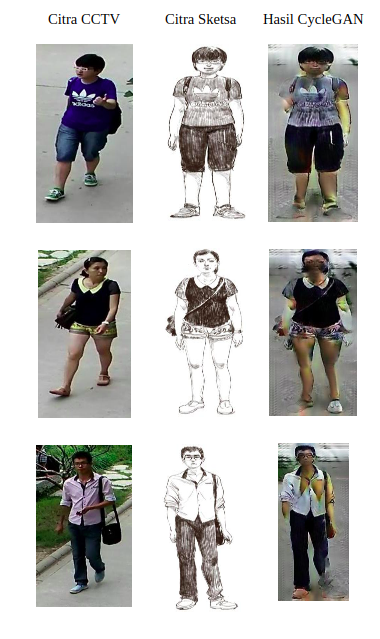
\includegraphics[scale=0.35]{img/CycleGANresults.png}
	\caption{Contoh hasil CycleGAN generasi ke 200}
	\label{fig: 3_3}
\end{figure}

Untuk CycleGAN nya sendiri, kami menggunakan model yang dibuat oleh Jun-Yan Zhu et al. dengan \textit{pre-trained weights} milik \textit{facades\_label2photo}. Citra yang digunakan untuk melatih gambar ini merupakan 600 citra yang terdapat pada dataset PKU Sketch Re-ID, dimana model ini di inisialisasi dengan \textit{learning rate} sebesar 0.0002 dan menurun ke 0.0001 setelah 150 epochs. Model CycleGAN ini kami \textit{train} selama 1000 epoch, namun kami memilih generasi ke 200 untuk dataset kami dikarenakan hasil sudah cukup baik.

\section{\textit{Local Binary Pattern}}
\vspace{1ex}
Salah satu cara lain yang kami gunakan untuk menjembatani perbedaan modalitas yang dimiliki oleh citra CCTV dan citra sketsa merupakan penggunaan \textit{Local Binary Pattern}. Dengan menggunakan \textit{Local Binary Pattern} dapat dilakukan pengambilan fitur tekstur dari citra CCTV, selain itu \textit{Local Binary Pattern} juga menggunakan citra hitam putih sehingga menyerupai citra sketsa yang ada.

\section{\textit{Training} dan \textit{Testing}}
\vspace{1ex}

\begin{figure}[h!] \centering
	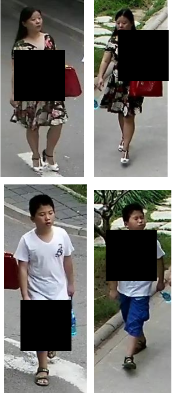
\includegraphics[width=0.28\textwidth]{img/RandomErasing.png}
	\caption{Contoh dari Random Erasing}
	\label{fig:4}
\end{figure}

Untuk memastikan bahwa kinerja model yang digunakan dapat diandalkan, kami melakukan proses training dan testing sebanyak 10 kali dan mengambil nilai rata-ratanya sebagai metrik evaluasi \textit{final}. Semua metode dievaluasi menggunakan akurasi Rank-1 milik model masing-masing, mengikuti ketentuan evaluasi yang ditentukan oleh Lu Pang et al.

\pagebreak

Pada eksperimen kami, kami mengatasi kurangnya data pada dataset PKU Sketch Re-Identification dengan cara melakukan \textit{pre-training} pada dataset Market-1501. Proses \textit{training} dilakukan selama 100 \textit{epochs}, dimana \textit{training} di inisialisasi dengan \textit{learning rate} sebesar 0,1 . \textit{Learning rate} tersebut akan berkurang dengan faktor  0.1 setiap 40 \textit{epochs}. Selain itu, kami melakukan \textit{random erasing} dan \textit{random crop} untuk menambahkan lebih banyak data \textit{training}. Gambar \ref{fig:4} menunjukan beberapa contoh dari augmentasi data yang dilakukan dengan metode \textit{Random Erasing}.

\section{Studi Ablasi}
\vspace{1ex}
Untuk memaksimalkan performa dari model ResNet-CIFAR yang digunakan, dilakukan studi ablasi dengan cara mengubah ukuran \textit{Fully Connected Layer} pertama yang digunakan oleh model. Ukuran \textit{Fully Connected Layer} yang digunakan adalah sebagai berikut; FC-128, FC-256, FC-512, FC-768, dan FC-1024. Selain itu dilakukan studi ablasi kedua dengan cara merubah probabilitas Random Erasing dari 0\% hingga 50\%. Pada pengujian ini kami hanya menggunakan model ResNet 56 dan ResNet 110 dikarenakan pada eksperimen sebelumnya kedua model tersebut mendapatkan rank-1 accuracy tertinggi dan kedua tertinggi.

\pagebreak

  \cleardoublepage

  % Bab 4 pengujian dan analisis
  \chapter{EKSPERIMEN DAN HASIL}
\label{chap:pengujiananalisis}

% Ubah bagian-bagian berikut dengan isi dari pengujian dan analisis

Pada penelitian ini dipaparkan hasil pengujian serta analisis dari desain sistem dan implementasi. Penggunaan dataset dari PKU Sketch Re-ID telah diambil dan telah meminta izin kepada \textit{National Engineering Laboratory for Video Technology}, Universitas Peking.
Pengujian ini dilakukan dalam empat bagian, yakni sebagai berikut:

\begin{enumerate}[nolistsep]
	\item Pengujian menggunakan Lightweight Residual Network
	\item Pengujian menggunakan Lightweight Residual Network \textit{pre-trained} pada Market-1501
	\item Pengujian menggunakan Re-Ranking
	\item Studi Ablasi
	\item Pengujian dengan menggunakan Ensemble.
	
	\vspace{1ex}
\end{enumerate}

Pada pengujian ini, pelatihan masing-masing model dilakukan dengan menggunakan laptop dengan spesifikasi \textit{hardware} sebagai berikut:

\begin{table}[h!]
	\begin{center}
		\begin{tabular}{|c|c|}
			\hline
			\textbf{Processor} & Intel(R) Core(TM) i7-8750H CPU @ 2.20GHz \\ \hline
			\textbf{RAM} & 8 GB DIMM DDR4 x 2\\ \hline
			\textbf{Storage} & HDD 512 GB \\ \hline
			\textbf{Graphics Card} & Nvidia GeForce GTX 1060 6GB MAX-Q \\ \hline
			\textbf{Operating System} & Ubuntu 18.04 LTS 64-bit \\ \hline
		\end{tabular}
	\end{center}
	\vspace{1ex}
	\caption{Spesifikasi Laptop yang digunakan}
	\label{tabel:3}
\end{table}


\section{Pengujian menggunakan Lightweight Residual Network}
\label{sec: nopretrained}
\vspace{1ex}
Pada pengujian ini, dilakukan \textit{training} dengan menggunakan Lightweight Residual Network, dimana pada model tidak dilakukan pelatihan ke dataset Market-1501 sebelum dilatih untuk melakukan klasifikasi pada dataset PKU Sketch Re-ID. Selain itu pada tahap pengujian ini dilakukan dua metode pengujian, yaitu dengan menggunakan metode Local Binary Pattern dan metode CycleGAN untuk menjembatani modalitas antara citra sketsa dan citra CCTV. Pada tahap pengujian ini hanya dilakukan pengujian pada model ResNet 20, pengujian seperti ini dilakukan karena model ini membutuhkan waktu \textit{training} paling sedikit dibandingkan dengan model \textit{lightweight} ResNet lain yang akan digunakan pada pengujian selanjutnya.

Tabel \ref{tabel: 4} menunjukan hasil dari training dan testing model sebanyak 10 kali untuk model ResNet 20 tanpa adanya perubahan pada dataset PKU Sketch Re-ID.

\vspace{1ex}

\begin{longtable}{|c|c|c|c|c|}
	\caption{Rata-rata performa ResNet 20}
	\label{tabel: 4}\\
	\hline
	\rowcolor[HTML]{C0C0C0}
	\textbf{No} &\textbf{Rank-1} & \textbf{Rank-5} & \textbf{Rank-10} & \textbf{mAP} \\
	\hline
	1 & 8 & 32 & 48 & 11.4505\\
	2 & 10 & 32 & 46 & 11.2543\\
	3 & 4 & 32 & 46 & 8.426\\
	4 & 8 & 24 & 32 & 9.842\\
	5 & 8 & 36 & 48 & 11.1407\\
	6 & 10 & 28 & 42 & 11.7093\\
	7 & 6 & 32 & 50 & 9.9849\\
	8 & 10 & 28 & 44 & 10.8898\\
	9 & 14 & 26 & 44 & 14.43\\
	10 & 8 & 26 & 42 & 10.3942\\
	\hline
	\textbf{Average} & 8.6 & 29.6 & 44.2 & 10.95217\\
	\hline
\end{longtable}

\vspace{1ex}

\subsection{\textit{Local Binary Pattern} (LBP)}

Tabel \ref{tabel: 5} menunjukan hasil dari training dan testing model sebanyak 10 kali untuk model ResNet 20 dengan menggunakan \textit{filter} LBP. Namun dikarenakan hasil yang didapatkan lebih rendah dibandingkan tanpa menggunakan LBP pada semua metrik evaluasi, sedangkan waktu yang dibutuhkan untuk \textit{training} menjadi 2 kali lebih banyak pengujian menggunakan LBP diberhentikan.

\begin{longtable}{|c|c|c|c|c|}
	\caption{Rata-rata performa ResNet 20 dengan Local Binary Pattern}
	\label{tabel: 5}\\
	\hline
	\rowcolor[HTML]{C0C0C0}
	\textbf{No} &\textbf{Rank-1} & \textbf{Rank-5} & \textbf{Rank-10} & \textbf{mAP} \\
	\hline
	1 & 2 & 30 & 40 & 7.7963\\
	2 & 4 & 26 & 44 & 8.898\\
	3 & 6 & 32 & 46 & 10.3007\\
	4 & 12 & 30 & 42 & 13.5232\\
	5 & 14 & 24 & 40 & 12.4012\\
	6 & 8 & 24 & 38 & 10.4669\\
	7 & 8 & 32 & 42 & 11.4641\\
	8 & 4 & 30 & 44 & 9.9319\\
	9 & 8 & 28 & 38 & 10.0783\\
	10 & 10 & 14 & 30 & 9.7921\\
	\hline
	\textbf{Average} & 7.6 & 27 & 40.4 & 10.46527\\
	\hline
\end{longtable}

\subsection{CycleGAN}

Tabel \ref{tabel: 6} menunjukan hasil dari training dan testing model sebanyak 10 kali untuk model ResNet 20 dimana citra sketsa pada dataset PKU Sketch Re-Identification telah dilakukan translasi \textit{style}.

\begin{longtable}{|c|c|c|c|c|}
	\caption{Rata-rata performa ResNet 20 dengan CycleGAN}
	\label{tabel: 6}\\
	\hline
	\rowcolor[HTML]{C0C0C0}
	\textbf{No} &\textbf{Rank-1} & \textbf{Rank-5} & \textbf{Rank-10} & \textbf{mAP} \\
	\hline
	1 & 8 & 16 & 34 & 8.9563\\
	2 & 12 & 28 & 36 & 14.2855\\
	3 & 10 & 24 & 40 & 10.558\\
	4 & 8 & 26 & 36 & 10.4396\\
	5 & 8 & 22 & 40 & 10.8883\\
	6 & 10 & 26 & 44 & 10.9954\\
	7 & 6 & 34 & 50 & 9.7\\
	8 & 14 & 28 & 42 & 13.4316\\
	9 & 8 & 26 & 42 & 10.5551\\
	10 & 10 & 26 & 38 & 12.737\\
	\hline
	\textbf{Average} & 9.4 & 25.6 & 40.2 & 11.25468\\
	\hline
\end{longtable}

Meskipun Rank-5 dan Rank-10 yang didapatkan lebih rendah, dikarenakan metrik evaluasi yang digunakan disamakan dengan pada paper "Cross-Domain Adversarial Feature Learning for Sketch Re-identification", yaitu menggunakan Rank-1 accuracy. Maka semua pengujian selanjutnya akan dilakukan menggunakan dataset yang telah ditranslasi dengan CycleGAN.

\section{Pengujian menggunakan Lightweight Residual Network \textit{pre-trained} pada Market-1501}
\label{sec:pretrained}

Pada pengujian ini dilakukan \textit{pre-training} terlebih dahulu pada dataset Market 1501 untuk mengatasi keterbatasan data pada dataset PKU Sketch Re-ID. Pada tahap pengujian ini, digunakan tiga jenis \textit{Lightweight Residual Network} yakni; ResNet 20, ResNet 56, dan ResNet 110. Dataset yang digunakan pada tahap pengujian ini semuanya merupakan hasil sintesis dari CycleGAN. 

\subsection{ResNet 20}

Tabel \ref{tabel: 7} menunjukan hasil dari training dan testing model sebanyak 10 kali untuk model ResNet 20 dengan model yang telah di \textit{pre-trained} pada dataset Market 1501 terlebih dahulu.

\vspace{1ex}

\begin{longtable}{|c|c|c|c|c|}
	\caption{Rata-rata performa ResNet 20 \textit{pretrained} pada Market 1501 }
	\label{tabel: 7}\\
	\hline
	\rowcolor[HTML]{C0C0C0}
	\textbf{No} &\textbf{Rank-1} & \textbf{Rank-5} & \textbf{Rank-10} & \textbf{mAP} \\
	\hline
	1 & 12 & 28 & 42 & 11.6169\\
	2 & 8 & 24 & 40 & 10.1131\\
	3 & 10 & 30 & 46 & 12.5311\\
	4 & 10 & 24 & 32 & 10.3256\\
	5 & 10 & 22 & 40 & 9.7441\\
	6 & 10 & 22 & 48 & 10.4837\\
	7 & 10 & 34 & 40 & 13.0863\\
	8 & 14 & 38 & 48 & 13.5198\\
	9 & 8 & 18 & 32 & 9.6554\\
	10 & 10 & 24 & 42 & 10.9248\\
	\hline
	\textbf{Average} & 10.2 & 26.4 & 41 & 11.30008\\
	\hline
\end{longtable}

\vspace{1ex}
Dapat dilihat terdapat peningkatan yang cukup signifikan pada Rank-1 accuracy yaitu dari 9,4\% ke 10,2\%. Selain itu Rank-5, Rank-10 , dan mAP yang didapatkan lebih tinggi dibandingkan pada saat tidak di \textit{pre-trained} pada Market 1501.

\subsection{ResNet56}

Tabel \ref{tabel: 8} menunjukan hasil dari training dan testing model sebanyak 10 kali untuk model ResNet 56 dengan model yang telah di \textit{pre-trained} pada dataset Market 1501 terlebih dahulu.

\vspace{1ex}

\begin{longtable}{|c|c|c|c|c|}
	\caption{Rata-rata performa ResNet 56 \textit{pretrained} pada Market 1501 }
	\label{tabel: 8}\\
	\hline
	\rowcolor[HTML]{C0C0C0}
	\textbf{No} &\textbf{Rank-1} & \textbf{Rank-5} & \textbf{Rank-10} & \textbf{mAP} \\
	\hline
	1 & 20 & 44 & 54 & 19.2315\\
	2 & 16 & 34 & 42 & 20.2117\\
	3 & 14 & 34 & 50 & 17.2698\\
	4 & 16 & 36 & 40 & 16.8498\\
	5 & 10 & 34 & 48 & 14.9505\\
	6 & 12 & 26 & 36 & 14.3816\\
	7 & 14 & 32 & 46 & 14.9699\\
	8 & 12 & 38 & 60 & 16.0066\\
	9 & 10 & 38 & 46 & 14.5599\\
	10 & 18 & 34 & 46 & 19.1052\\
	\hline
	\textbf{Average} & 14.2 & 35 & 47.8 & 16.95365\\
	\hline
\end{longtable}

Terlihat terdapat peningkatan yang sangat signifikan pada Rank-1, yaitu sebesar 40\% apabila dibandingkan dengan ResNet 20.

\subsection{ResNet 110}

Tabel \ref{tabel: 9} menunjukan hasil dari training dan testing model sebanyak 10 kali untuk model ResNet 110 dengan model yang telah di \textit{pre-trained} pada dataset Market 1501 terlebih dahulu. Pada pengujian ini terlihat terdapat peningkatan yang sangat signifikan pada Rank-1, yaitu sebesar 70\% apabila dibandingkan dengan ketika menggunakan model ResNet 20.

\vspace{1ex}

\begin{longtable}{|c|c|c|c|c|}
	\caption{Rata-rata performa ResNet 110 \textit{pretrained} pada Market 1501 }
	\label{tabel: 9}\\
	\hline
	\rowcolor[HTML]{C0C0C0}
	\textbf{No} &\textbf{Rank-1} & \textbf{Rank-5} & \textbf{Rank-10} & \textbf{mAP} \\
	\hline
	1 & 18 & 36 & 56 & 17.9811\\
	2 & 20 & 46 & 62 & 21.6104\\
	3 & 18 & 40 & 56 & 19.7356\\
	4 & 16 & 44 & 54 & 18.3177\\
	5 & 18 & 46 & 56 & 18.1901\\
	6 & 16 & 38 & 42 & 17.9401\\
	7 & 18 & 36 & 54 & 20.0548\\
	8 & 16 & 38 & 52 & 18.2794\\
	9 & 12 & 26 & 38 & 14.3971\\
	10 & 22 & 38 & 52 & 22.2614\\
	\hline
	\textbf{Average} & 17.4 & 38.8 & 52.2 & 18.87587\\
	\hline
\end{longtable}
\vspace{2ex}
\section{Pengujian menggunakan Re-Ranking}
\vspace{2ex}
Pada tahap pengujian ini dilakukan Re-Ranking pada hasil training dan testing 10 kali yang telah dilakukan pada model Residual Network 56 dan 110. Re-Ranking dilakukan dengan harapan dapat meningkatkan performa Rank-1 model, dikarenakan dari penelitian re-identifikasi orang, dapat dilihat bahwa \textit{re-ranking} dapat meningkatkan performa Rank-1 dan mAP model.
\vspace{2ex}
\subsection{Re-Ranking pada ResNet 56}
\vspace{2ex}
Pada tahap pengujian ini dilakukan re-ranking terhadap 10 metrik evaluasi yang tertera pada tabel \ref{tabel: 8}, dimana reranking merupakan pengambilan jarak antara citra query dan citra gallery yang terdekat. Dapat dilihat pada hasil \textit{re-ranking} di tabel \ref{tabel:10}, bahwa semua metrik evaluasi yang digunakan menurun drastis. Yaitu masing-masing sebesar 6.2\% , 9.6\%, 5\%, dan 0.18\%. Hal ini menunjukan bahwa re-identifikasi sketsa merupakan sebuah permasalahan yang sangat berbeda dengan re-identifikasi manusia.

\begin{longtable}{|c|c|c|c|c|}
	\caption{Rata-rata performa ResNet 56 dengan re-ranking}
	\label{tabel:10}\\
	\hline
	\rowcolor[HTML]{C0C0C0}
	\textbf{No} &\textbf{Rank-1} & \textbf{Rank-5} & \textbf{Rank-10} & \textbf{mAP} \\
	\hline
	1 &8 &26 &34 &10.5473 \\
	2 &8 &28 &38 &11.8655 \\
	3 &6 &28 &38 &10.9266 \\
	4 &8 &22 &30 &10.9797 \\
	5 &8 &20 &34 &11.7746 \\
	6 &6 &26 &34 &10.4775 \\
	7 &6 &26 &36 &10.8615 \\
	8 &10 &26 &34 &12.5916 \\
	9 &6 &26 &38 &10.3757 \\
	10 &14 &26 &44 &14.4551 \\
	\hline
	\textbf{Average} & 8 & 25.4 & 36 &11.48551 \\
	\hline
\end{longtable}

\subsection{Re-Ranking pada ResNet 110}
\vspace{2ex}
Sama dengan pada Residual Network 56 dapat dilihat bahwa re-ranking menyebabkan terjadinya penurunan pada semua metrik evaluasi.

\begin{longtable}{|c|c|c|c|c|}
	\caption{Rata-rata performa ResNet 110 dengan re-ranking}
	\label{tabel:11}\\
	\hline
	\rowcolor[HTML]{C0C0C0}
	\textbf{No} &\textbf{Rank-1} & \textbf{Rank-5} & \textbf{Rank-10} & \textbf{mAP} \\
	\hline
	1 &8 &24 &40 &12.0668 \\
	2 &10 &34 &36 &13.4624 \\
	3 &6 &24 &34 &10.1525 \\
	4 &10 &26 &38 &14.866 \\
	5 &16 &32 &46 &17.1341 \\
	6 &10 &20 &26 &12.8491 \\
	7 &14 &30 &36 &16.3645 \\
	8 &18 &30 &42 &19.7371 \\
	9 &6 &22 &36 &9.6301 \\
	10 &8 &24 &38 &10.146 \\
	\hline
	\textbf{Average} & 10.6 & 26.6 & 37.2 &13.640859 \\
	\hline
\end{longtable}

\pagebreak

\subsection{Kesimpulan Re-Ranking untuk Re-Identifikasi Sketsa}
Dari pengujian yang dilakukan pada kedua model, dapat dilihat bahwa \textit{re-ranking} yang dilakukan menyebabkan penurunan performa yang sangat drastis pada kedua model. Selain itu dapat dilihat bahwa pada semua metrik evaluasi, tidak ada yang meningkat, berbeda dengan pada re-identifikasi manusia dimana Rank-1 dan mean Average Precision meningkat. Oleh karena hasil yang kami dapatkan sebagai berikut maka percobaan dengan \textit{re-ranking} tidak akan dilanjutkan lebih lagi. Tabel dibawah menunjukkan perbedaan performa rata-rata dari kedua model dengan hasil re-rankingnya.

\section{Pengujian menggunakan Re-Ranking}
\vspace{2ex}
Pada tahap pengujian ini dilakukan Re-Ranking pada hasil training dan testing 10 kali yang telah dilakukan pada model Residual Network 56 dan 110. Re-Ranking dilakukan dengan harapan dapat meningkatkan performa Rank-1 model, dikarenakan dari penelitian re-identifikasi orang, dapat dilihat bahwa \textit{re-ranking} dapat meningkatkan performa Rank-1 dan mAP model.
\vspace{2ex}
\subsection{Re-Ranking pada ResNet 56}
\vspace{2ex}
Pada tahap pengujian ini dilakukan re-ranking terhadap 10 metrik evaluasi yang tertera pada tabel \ref{tabel: 8}, dimana reranking merupakan pengambilan jarak antara citra query dan citra gallery yang terdekat. Dapat dilihat pada hasil \textit{re-ranking} di tabel \ref{tabel:10}, bahwa semua metrik evaluasi yang digunakan menurun drastis. Yaitu masing-masing sebesar 6.2\% , 9.6\%, 5\%, dan 0.18\%. Hal ini menunjukan bahwa re-identifikasi sketsa merupakan sebuah permasalahan yang sangat berbeda dengan re-identifikasi manusia.

\pagebreak

\begin{longtable}{|c|c|c|c|c|}
	\caption{Rata-rata performa ResNet 56 dengan re-ranking}
	\label{tabel:10}\\
	\hline
	\rowcolor[HTML]{C0C0C0}
	\textbf{No} &\textbf{Rank-1} & \textbf{Rank-5} & \textbf{Rank-10} & \textbf{mAP} \\
	\hline
	1 &8 &26 &34 &10.5473 \\
	2 &8 &28 &38 &11.8655 \\
	3 &6 &28 &38 &10.9266 \\
	4 &8 &22 &30 &10.9797 \\
	5 &8 &20 &34 &11.7746 \\
	6 &6 &26 &34 &10.4775 \\
	7 &6 &26 &36 &10.8615 \\
	8 &10 &26 &34 &12.5916 \\
	9 &6 &26 &38 &10.3757 \\
	10 &14 &26 &44 &14.4551 \\
	\hline
	\textbf{Average} & 8 & 25.4 & 36 &11.48551 \\
	\hline
\end{longtable}

\subsection{Re-Ranking pada ResNet 110}
\vspace{2ex}
Sama dengan pada Residual Network 56 dapat dilihat bahwa re-ranking menyebabkan terjadinya penurunan pada semua metrik evaluasi.

\begin{longtable}{|c|c|c|c|c|}
	\caption{Rata-rata performa ResNet 110 dengan re-ranking}
	\label{tabel:11}\\
	\hline
	\rowcolor[HTML]{C0C0C0}
	\textbf{No} &\textbf{Rank-1} & \textbf{Rank-5} & \textbf{Rank-10} & \textbf{mAP} \\
	\hline
	1 &8 &24 &40 &12.0668 \\
	2 &10 &34 &36 &13.4624 \\
	3 &6 &24 &34 &10.1525 \\
	4 &10 &26 &38 &14.866 \\
	5 &16 &32 &46 &17.1341 \\
	6 &10 &20 &26 &12.8491 \\
	7 &14 &30 &36 &16.3645 \\
	8 &18 &30 &42 &19.7371 \\
	9 &6 &22 &36 &9.6301 \\
	10 &8 &24 &38 &10.146 \\
	\hline
	\textbf{Average} & 10.6 & 26.6 & 37.2 &13.640859 \\
	\hline
\end{longtable}

\pagebreak

\subsection{Kesimpulan Re-Ranking untuk Re-Identifikasi Sketsa}
Dari pengujian yang dilakukan pada kedua model, dapat dilihat bahwa \textit{re-ranking} yang dilakukan menyebabkan penurunan performa yang sangat drastis pada kedua model. Selain itu dapat dilihat bahwa pada semua metrik evaluasi, tidak ada yang meningkat, berbeda dengan pada re-identifikasi manusia dimana Rank-1 dan mean Average Precision meningkat. Oleh karena hasil yang kami dapatkan sebagai berikut maka percobaan dengan \textit{re-ranking} tidak akan dilanjutkan lebih lagi. Tabel dibawah menunjukkan perbedaan performa rata-rata dari kedua model dengan hasil re-rankingnya.

\begin{table}[h!]
	\begin{center}
		\begin{tabular}{|c|c|c|c|c|}
			\hline
			\textbf{Name} & \textbf{Rank-1} & \textbf{Rank-5} & \textbf{Rank-10} & \textbf{mAP} \\ \hline
			ResNet 56 & 14.2\% & 35\% & 47.8\% & 16.95\%\\ \hline
			ResNet 56 + re-rank  & 8\% & 25.4\% & 36\% & 11.49\%\\ \hline
			ResNet 110 & 17.4\% & 38.8\% & 52.2\% & 18.88\%\\ \hline
			ResNet 110 + re-rank & 10.6\% & 26.6\% & 37.2\% & 13.64\%\\ \hline
		\end{tabular}
	\end{center}
\end{table}
\vspace{-3ex}
\section{Studi Ablasi}
\subsection{Perubahan pada Fully Connected Layer}
\vspace{1ex}

Pada tahap pengujian ini dilakukan perubahan \textit{Fully Connected layer} pertama yang terdapat pada ResNet 56 dan ResNet 110. Studi Ablasi hanya dilakukan pada kedua model tersebut dikarenakan terjadi peningkatan yang sangat signifikan dibanding dengan menggunakan ResNet 20, yaitu 40\% dan 70\%. Pengujian ini dilakukan dengan 5 jenis \textit{Fully Connected Layer} yaitu:

\begin{enumerate}[nolistsep]
	\item \textit{Fully Connected} 128
	\item \textit{Fully Connected} 256
	\item \textit{Fully Connected} 512
	\item \textit{Fully Connected} 768
	\item \textit{Fully Connected} 1024
	\vspace{1ex}
\end{enumerate}

Semua pengujian sebelumnya dilakukan dengan \textit{Fully Connected layer} sebesar 512. Oleh karena itu, pada bagian ini dilakukan pengujian pada Fully Connected lainnya yang tertera.

\pagebreak

\subsection{ResNet 56 Fully Connected 128}
\vspace{1ex}
\begin{longtable}{|c|c|c|c|c|}
	\caption{Rata-rata performa ResNet 56 Fully Connected 128 \textit{pretrained} pada Market 1501}
	\label{tabel: 10}\\
	\hline
	\rowcolor[HTML]{C0C0C0}
	\textbf{No} &\textbf{Rank-1} & \textbf{Rank-5} & \textbf{Rank-10} & \textbf{mAP} \\
	\hline
	1 &8 &42 &52 &13.4307 \\
	2 &14 &36 &48 &15.8562 \\
	3 &12 &28 &40 &13.4272 \\
	4 &10 &34 &50 &15.0407 \\
	5 &10 &34 &46 &13.7825 \\
	6 &10 &38 &58 &15.3561 \\
	7 &12 &36 &50 &17.1585 \\
	8 &14 &38 &50 &16.2073 \\
	9 &10 &42 &58 &16.2594 \\
	10 &14 &36 &48 &17.6873 \\
	\hline
	\textbf{Average} & 11.4 & 36.4 & 50 &15.42059 \\
	\hline
\end{longtable}
\vspace{2ex}
	Pada penggunaaan Fully Connected Layer sebesar 128, terjadi penurunan pada Rank-1 accuracy sebesar 2.8\% apabila dibandingkan dengan 512 layer. Selain itu Rank-5 dan mean Average Precision yang didapatkan kedua nya lebih rendah apabila dibandingkan dengan 512 layer, yaitu masing masing mendapatkan penurunan sebesar 2.2\% dan 1.53306\%.
\vspace{2ex}
\subsection{ResNet 56 Fully Connected 256}
\vspace{1ex}
Pada penggunaaan Fully Connected Layer sebesar 256, terjadi penurunan pada Rank-1 accuracy sebesar 1.4\% apabila dibandingkan dengan 512 layer. Selain itu Rank-5, Rank-10 dan mean Average Precision yang didapatkan semuanya mendapatkan hasil yang lebih rendah apabila dibandingkan dengan 512 layer. 

Dari dua percobaan ini dapat disimpulkan bahwa menggunakan layer dibawah 512 tidak seefektif menggunakan 512 layer dikarenakan adanya informasi yang hilang yang diakibatkan oleh serialisasi data yang dilakukan oleh adanya Fully Connected Layer.

\begin{longtable}{|c|c|c|c|c|}
	\caption{Rata-rata performa ResNet 56 Fully Connected 256 \textit{pretrained} pada Market 1501}
	\label{tabel: 11}\\
	\hline
	\rowcolor[HTML]{C0C0C0}
	\textbf{No} &\textbf{Rank-1} & \textbf{Rank-5} & \textbf{Rank-10} & \textbf{mAP} \\
	\hline
	1 &16 &32 &48 &16.7992 \\
	2 &14 &32 &48 &17.5719 \\
	3 &14 &26 &40 &15.5429 \\
	4 &12 &26 &46 &14.9202 \\
	5 &12 &30 &50 &14.5889 \\
	6 &10 &32 &52 &13.3994 \\
	7 &8 &28 &44 &12.6595 \\
	8 &10 &36 &48 &16.2244 \\
	9 &16 &38 &54 &18.6509 \\
	10 &16 &38 &50 &16.84 \\
	\hline
	\textbf{Average} & 12.8 & 31.8 & 48 &15.7197299 \\
	\hline
\end{longtable}

\subsection{ResNet 56 Fully Connected 768}
Pada penggunaaan FC Layer sebesar 768, terjadi penurunan pada rank1 accuracy sebesar 0.4\% apabila dibandingkan dengan 512 layer.

\begin{longtable}{|c|c|c|c|c|}
	\caption{Rata-rata performa ResNet 56 Fully Connected 768 \textit{pretrained} pada Market 1501}
	\label{tabel: 12}\\
	\hline
	\rowcolor[HTML]{C0C0C0}
	\textbf{No} &\textbf{Rank-1} & \textbf{Rank-5} & \textbf{Rank-10} & \textbf{mAP} \\
	\hline
	1 &8 &44 &48 &13.5317 \\
	2 &16 &36 &50 &16.791 \\
	3 &12 &38 &54 &15.9576 \\
	4 &14 &32 &42 &16.0422 \\
	5 &10 &34 &44 &13.8197 \\
	6 &18 &26 &54 &19.7984 \\
	7 &14 &40 &48 &19.3302 \\
	8 &14 &34 &44 &15.6428 \\
	9 &18 &38 &44 &17.7032 \\
	10 &14 &36 &40 &16.417 \\
	\hline
	\textbf{Average} & 13.8 & 35.8 & 46.8 &16.50338 \\
	\hline
\end{longtable}

 Namun Rank-5 yang didapatkan lebih tinggi apabila dibandingkan dengan menggunakan 512 layer. Penurunan performa ini dapat terjadi dikarenakan adanya overfitting yang disebabkan oleh penambahan Fully Connected Layer, sehingga performa dari model tidak stabil.

\subsection{ResNet 56 Fully Connected 1024}
\vspace{2ex}
\begin{longtable}{|c|c|c|c|c|}
	\caption{Rata-rata performa ResNet 56 Fully Connected 1024 \textit{pretrained} pada Market 1501 }
	\label{tabel: 13}\\
	\hline
	\rowcolor[HTML]{C0C0C0}
	\textbf{No} &\textbf{Rank-1} & \textbf{Rank-5} & \textbf{Rank-10} & \textbf{mAP} \\
	\hline
	1 &14 &32 &48 &15.9998 \\
	2 &18 &46 &58 &18.8938 \\
	3 &14 &28 &52 &16.1321 \\
	4 &24 &36 &48 &21.9224 \\
	5 &10 &30 &44 &15.1594 \\
	6 &18 &36 &56 &18.5048 \\
	7 &14 &40 &50 &18.6785 \\
	8 &14 &40 &52 &19.3363 \\
	9 &12 &36 &52 &15.2779 \\
	10 &12 &32 &50 &15.9013 \\
	\hline
	\textbf{Average} & 15 & 35.6 & 51 &17.58063 \\
	\hline
\end{longtable}
\vspace{2ex}
Pada penggunaaan FC Layer sebesar 1024, terjadi peningkatan pada Rank-1 accuracy sebesar 0.8\% apabila dibandingkan dengan 512 layer. Selain itu performa yang didapatkan pada Rank-5, Rank-10, dan mAP semua mendapatkan peningkatan performa, yaitu masing-masing sebanyak 0.6\%, 3.2\%, dan 0.62\%.

\subsection{Kesimpulan FC Layer pada ResNet 56}
Dari semua pengujian yang dilakukan dapat dilihat bahwa pengujian naik perlahan dari Fully Connected layer 128, 256, 512. Namun pada saat mencapat 768 layer, performa dari model menjadi tidak stabil dan naik turun. Hal tersebut dapat dilihat dari rata-rata 10 kali pengujian pada 768 layer dan 1024 layer.

\subsection{ResNet 110 Fully Connected 128}

\begin{longtable}{|c|c|c|c|c|}
	\caption{Rata-rata performa ResNet 110 Fully Connected 128 \textit{pretrained} pada Market 1501 }
	\label{tabel: 14}\\
	\hline
	\rowcolor[HTML]{C0C0C0}
	\textbf{No} &\textbf{Rank-1} & \textbf{Rank-5} & \textbf{Rank-10} & \textbf{mAP} \\
	\hline
	1 &14 &36 &54 &16.5342 \\
	2 &12 &34 &50 &15.9617 \\
	3 &16 &38 &50 &17.08 \\
	4 &12 &34 &48 &15.1201 \\
	5 &12 &32 &40 &14.5804 \\
	6 &10 &34 &50 &13.7103 \\
	7 &12 &42 &50 &15.9939 \\
	8 &14 &38 &46 &15.9738 \\
	9 &16 &32 &44 &16.66048 \\
	10 &12 &38 &58 &16.5114 \\
	\hline
	\textbf{Average} & 13 & 35.8 & 49 &15.812628 \\
	\hline
\end{longtable}
	Pada penggunaaan Fully Connected Layer sebesar 128, terjadi penurunan pada Rank-1 accuracy sebesar 4.4\% apabila dibandingkan dengan 512 layer. Selain itu Rank-5, Rank-10 dan mean Average Precision yang didapatkan semua nya lebih rendah apabila dibandingkan dengan 512 layer, yaitu masing masing mendapatkan penurunan sebesar 3\%, 3.2\%, dan 3.06\%.
	
\subsection{ResNet 110 Fully Connected 256}
Pada penggunaaan Fully Connected Layer sebesar 256, terjadi penurunan pada Rank-1 accuracy sebesar 3.6\% apabila dibandingkan dengan 512 layer. Selain itu Rank-5 dan mean Average Precision yang didapatkan mendapatkan hasil yang lebih rendah apabila dibandingkan dengan 512 layer. 

Dari dua percobaan ini dapat disimpulkan bahwa menggunakan layer dibawah 512 tidak seefektif menggunakan 512 layer dikarenakan adanya informasi yang hilang yang diakibatkan oleh serialisasi data yang dilakukan oleh adanya Fully Connected Layer.
\begin{longtable}{|c|c|c|c|c|}
	\caption{Rata-rata performa ResNet 110 Fully Connected 256 \textit{pretrained} pada Market 1501 }
	\label{tabel: 15}\\
	\hline
	\rowcolor[HTML]{C0C0C0}
	\textbf{No} &\textbf{Rank-1} & \textbf{Rank-5} & \textbf{Rank-10} & \textbf{mAP} \\
	\hline
	1 &14 &34 &46 &15.2228 \\
	2 &10 &38 &54 &14.5828 \\
	3 &16 &36 &50 &19.2416 \\
	4 &20 &42 &54 &21.7159 \\
	5 &12 &32 &56 &15.9766 \\
	6 &10 &44 &56 &14.7769 \\
	7 &12 &38 &54 &15.1684 \\
	8 &12 &38 &54 &16.4656 \\
	9 &16 &40 &50 &17.2462 \\
	10 &16 &42 &54 &18.3998 \\
	\hline
	\textbf{Average} & 13.8 & 38.4 & 52.8 &16.87965999 \\
	\hline
\end{longtable}

\subsection{ResNet 110 Fully Connected 768}

Pada penggunaaan FC Layer sebesar 768, terjadi penurunan pada Rank-1 accuracy sebesar 3\% apabila dibandingkan dengan 512 layer.
\begin{longtable}{|c|c|c|c|c|}
	\caption{Rata-rata performa ResNet 110 Fully Connected 768 \textit{pretrained} pada Market 1501 }
	\label{tabel: 16}\\
	\hline
	\rowcolor[HTML]{C0C0C0}
	\textbf{No} &\textbf{Rank-1} & \textbf{Rank-5} & \textbf{Rank-10} & \textbf{mAP} \\
	\hline
	1 &18 &44 &60 &18.9191 \\
	2 &16 &40 &48 &17.0235 \\
	3 &14 &36 &52 &15.8576 \\
	4 &12 &38 &54 &16.2625 \\
	5 &16 &36 &48 &19.3128 \\
	6 &14 &34 &42 &18.631 \\
	7 &14 &36 &44 &15.2293 \\
	8 &12 &30 &38 &12.5104 \\
	9 &16 &38 &56 &17.084 \\
	10 &12 &36 &46 &14.0698 \\
	\hline
	\textbf{Average} & 14.4 & 36.8 & 48.8 &16.49 \\
	\hline
\end{longtable}
 Namun Rank-5 yang didapatkan lebih tinggi apabila dibandingkan dengan menggunakan 512 layer. Penurunan performa ini dapat terjadi dikarenakan adanya overfitting yang disebabkan oleh penambahan Fully Connected Layer, sehingga performa dari model tidak stabil, sama seperti pada ResNet 56.

\subsection{ResNet 110 Fully Connected 1024}
\begin{longtable}{|c|c|c|c|c|}
	\caption{Rata-rata performa ResNet 110 Fully Connected 1024 \textit{pretrained} pada Market 1501 }
	\label{tabel: 17}\\
	\hline
	\rowcolor[HTML]{C0C0C0}
	\textbf{No} &\textbf{Rank-1} & \textbf{Rank-5} & \textbf{Rank-10} & \textbf{mAP} \\
	\hline
	1 &10 &36 &50 &14.307 \\
	2 &16 &40 &52 &18.0064 \\
	3 &20 &42 &58 &21.334 \\
	4 &16 &42 &52 &16.4967 \\
	5 &22 &48 &60 &25.3244 \\
	6 &12 &34 &50 &15.2809 \\
	7 &20 &36 &62 &21.1675 \\
	8 &16 &34 &46 &17.2766 \\
	9 &14 &48 &60 &16.4865 \\
	10 &12 &30 &44 &14.861 \\
	\hline
	\textbf{Average} & 15.8 & 39 & 53.4 &18.0541 \\
	\hline
\end{longtable}
Pada penggunaaan FC Layer sebesar 1024, terjadi penurunan pada Rank-1 accuracy sebesar 1.6\% apabila dibandingkan dengan 512 layer. Namun performa yang didapatkan pada Rank-5, Rank-10 mendapatkan peningkatan performa, yaitu masing-masing sebanyak 0.2\%, 1.2\%.

\subsection{Kesimpulan FC Layer pada ResNet 110}
Dari semua pengujian yang dilakukan dapat dilihat bahwa pengujian naik perlahan dari Fully Connected layer 128, 256, 512. Namun pada saat mencapat 768 layer, terjadi overfitting pada model sehingga performa model turun perlahan.

\pagebreak
\subsection{Perubahan pada Probabilitas \textit{Random Erasing}}
Pada tahap pengujian ini dilakukan perubahan probabilitas \textit{Random Erasing}, dimana pengujian ini dilakukan dengan 6 jenis \textit{Random Erasing} yaitu:

\begin{enumerate}[nolistsep]
	\item \textit{Random Erasing} 0\%
	\item \textit{Random Erasing} 10\%
	\item \textit{Random Erasing} 20\%
	\item \textit{Random Erasing} 30\%
	\item \textit{Random Erasing} 40\%
	\item \textit{Random Erasing} 50\%
	\vspace{1ex}
\end{enumerate}
Namun dikarenakan pengujian sebelumnya telah dilakukan dengan Random Erasing 50\%, maka hanya pengujian tersisa yang dituliskan.

\subsection{ResNet 56 \textit{Random Erasing} 0\%}
\begin{longtable}{|c|c|c|c|c|}
	\caption{Rata-rata performa ResNet 56 Random Erasing 0\%}
	\label{tabel: 30}\\
	\hline
	\rowcolor[HTML]{C0C0C0}
	\textbf{No} &\textbf{Rank-1} & \textbf{Rank-5} & \textbf{Rank-10} & \textbf{mAP} \\
	\hline
	1 &18 &36 &56 &19.2064 \\
	2 &14 &38 &50 &17.4292 \\
	3 &18 &38 &46 &21.0595 \\
	4 &20 &36 &62 &22.4735 \\
	5 &18 &38 &52 &20.4456 \\
	6 &20 &36 &50 &21.4024 \\
	7 &10 &28 &42 &13.1137 \\
	8 &14 &36 &50 &19.71 \\
	9 &14 &40 &50 &18.1666 \\
	10 &16 &38 &48 &18.4812 \\
	\hline
	\textbf{Average} & 16.2 & 36.4 & 50.6 &19.14881 \\
	\hline
\end{longtable}

Performa dari model yang dibuat lebih baik dibandingkan dengan menggunakan Random Erasing 50\%. Dimana pada Rank-1 yang didapatkan terdapat peningkatan sebesar 2\%, selain itu Rank-5, Rank-10, dan mAP yang didapatkan semuanya lebih tinggi.

\subsection{ResNet 56 \textit{Random Erasing} 10\%}

\begin{longtable}{|c|c|c|c|c|}
	\caption{Rata-rata performa ResNet 56 Random Erasing 10\%}
	\label{tabel: 31}\\
	\hline
	\rowcolor[HTML]{C0C0C0}
	\textbf{No} &\textbf{Rank-1} & \textbf{Rank-5} & \textbf{Rank-10} & \textbf{mAP} \\
	\hline
	1 &14 &36 &50 &18.2589 \\
	2 &12 &48 &56 &17.2826 \\
	3 &16 &30 &44 &18.0019 \\
	4 &22 &44 &60 &24.5899 \\
	5 &10 &34 &52 &18.5679 \\
	6 &14 &38 &48 &17.2811 \\
	7 &10 &46 &58 &16.8315 \\
	8 &14 &30 &54 &17.3568 \\
	9 &14 &36 &48 &16.2783 \\
	10 &20 &46 &54 &22.2397 \\
	\hline
	\textbf{Average} & 14.6 & 38.8 & 52.4 &18.66886 \\
	\hline
\end{longtable}
\vspace{-1ex}
Pada penggunaaan Random Erasing sebesar 10\%, rank1 accuracy menurun sebesar 2\% apabila dibandingkan dengan ketika tidak dilakukan Random Erasing. Selain itu metrik evaluasi yang didapatkan semua nya lebih rendah dari pengujian sebelumnya. 
\subsection{ResNet 56 \textit{Random Erasing} 20\%}
\begin{longtable}{|c|c|c|c|c|}
	\caption{Rata-rata performa ResNet 56 Random Erasing 20\%}
	\label{tabel: 32}\\
	\hline
	\rowcolor[HTML]{C0C0C0}
	\textbf{No} &\textbf{Rank-1} & \textbf{Rank-5} & \textbf{Rank-10} & \textbf{mAP} \\
	\hline
	1 &14 &32 &50 &15.9493 \\
	2 &16 &36 &44 &17.8214 \\
	3 &12 &28 &52 &16.0317 \\
	4 &10 &36 &48 &15.425 \\
	5 &20 &44 &52 &22.233 \\
	6 &14 &36 &48 &16.2473 \\
	7 &14 &34 &48 &18.1056 \\
	8 &14 &48 &62 &18.3149 \\
	9 &12 &36 &58 &16.9772 \\
	10 &16 &42 &50 &21.1495 \\
	\hline
	\textbf{Average} & 14.2 & 37.2 & 51.2 &17.82549 \\
	\hline
\end{longtable}

Pada penggunaaan Random Erasing sebesar 20\%, terjadi penurunan pada Rank-1 accuracy sebesar 2.4\% apabila dibandingkan dengan tanpa menggunakan Random Erasing. Selain itu Rank-5, Rank-10 dan mean Average Precision yang didapatkan semuanya mendapatkan hasil yang lebih rendah apabila dibandingkan dengan pengujian sebelumnya. 

Dari tiga percobaan ini dapat disimpulkan bahwapenggunaan Random Erasing mengurangi efektifitas model, dimana dapat dilihat bahwa performa model turun sangat signifikan dari tanpa menggunakan Random Erasing ke menggunakan Random Erasing sebesar 10\%.

\subsection{ResNet 56 \textit{Random Erasing} 30\%}

Pada penggunaaan Random Erasing sebesar 30\%, terjadi penurunan pada Rank-1 accuracy sebesar 3.4\% apabila dibandingkan dengan tanpa menggunakan Random Erasing.

\begin{longtable}{|c|c|c|c|c|}
	\caption{Rata-rata performa ResNet 56 Random Erasing 30\%}
	\label{tabel: 33}\\
	\hline
	\rowcolor[HTML]{C0C0C0}
	\textbf{No} &\textbf{Rank-1} & \textbf{Rank-5} & \textbf{Rank-10} & \textbf{mAP} \\
	\hline
	1 &12 &34 &44 &18.1763 \\
	2 &18 &34 &42 &18.8824 \\
	3 &14 &32 &60 &16.3065 \\
	4 &10 &22 &38 &13.5783 \\
	5 &10 &32 &46 &14.0838 \\
	6 &22 &32 &50 &22.304 \\
	7 &4 &38 &50 &11.7184 \\
	8 &8 &28 &46 &13.8258 \\
	9 &10 &28 &38 &14.577 \\
	10 &20 &42 &50 &21.7607 \\
	\hline
	\textbf{Average} & 12.8 & 32.2 & 46.4 &16.5213199 \\
	\hline
\end{longtable}
Selain itu terjadi penurunan performa di semua metrik evaluasi lainnya. Penurunan performa ini dapat terjadi dikarenakan adanya underfitting yang disebabkan oleh terlalu banyaknya data yang dihapus oleh Random Erasing.

\subsection{ResNet 56 \textit{Random Erasing} 40\%}

\begin{longtable}{|c|c|c|c|c|}
	\caption{Rata-rata performa ResNet 56 Random Erasing 40\%}
	\label{tabel: 34}\\
	\hline
	\rowcolor[HTML]{C0C0C0}
	\textbf{No} &\textbf{Rank-1} & \textbf{Rank-5} & \textbf{Rank-10} & \textbf{mAP} \\
	\hline
	1 &10 &32 &50 &14.6807 \\
	2 &10 &40 &54 &15.7018 \\
	3 &18 &34 &46 &18.469 \\
	4 &8 &42 &56 &14.5516 \\
	5 &14 &34 &48 &17.6434 \\
	6 &18 &32 &50 &19.003 \\
	7 &12 &32 &44 &17.2603 \\
	8 &12 &40 &50 &15.8508 \\
	9 &18 &36 &48 &19.563 \\
	10 &14 &38 &48 &17.0508 \\
	\hline
	\textbf{Average} & 13.4 & 36 & 49.4 &16.97744 \\
	\hline
\end{longtable}

Terjadi peningkatan performa apabila dibandingkan dengan percobaan sebelumnya, peningkatan performa ini dapat terjadi dikarenakan probabilitas Random Erasing cukup besar sehingga performa model tidak konsisten.

\subsection{ResNet 110 \textit{Random Erasing} 0\%}
\begin{longtable}{|c|c|c|c|c|}
	\caption{Rata-rata performa ResNet 110 Random Erasing 0\%}
	\label{tabel: 36}\\
	\hline
	\rowcolor[HTML]{C0C0C0}
	\textbf{No} &\textbf{Rank-1} & \textbf{Rank-5} & \textbf{Rank-10} & \textbf{mAP} \\
	\hline
	1 &14 &30 &42 &16.4663 \\
	2 &24 &40 &46 &22.5784 \\
	3 &16 &34 &48 &17.7241 \\
	4 &20 &34 &44 &20.0728 \\
	5 &22 &44 &56 &23.8577 \\
	6 &24 &38 &42 &23.8481 \\
	7 &24 &36 &52 &22.8688 \\
	8 &20 &40 &56 &22.4153 \\
	9 &16 &38 &50 &19.2107 \\
	10 &18 &40 &42 &21.3032 \\
	\hline
	\textbf{Average} & 19.8 & 37.4 & 47.8 &21.03454 \\
	\hline
\end{longtable}

Performa dari model yang dibuat lebih baik dibandingkan dengan menggunakan Random Erasing 50\%. Dimana pada Rank-1 yang didapatkan terdapat peningkatan sebesar 2\%, selain itu Rank-5, Rank-10, dan mAP yang didapatkan semuanya lebih tinggi.

\subsection{ResNet 110 \textit{Random Erasing} 10\%}

\begin{longtable}{|c|c|c|c|c|}
	\caption{Rata-rata performa ResNet 110 Random Erasing 20\%}
	\label{tabel: 31}\\
	\hline
	\rowcolor[HTML]{C0C0C0}
	\textbf{No} &\textbf{Rank-1} & \textbf{Rank-5} & \textbf{Rank-10} & \textbf{mAP} \\
	\hline
	1 &18 &38 &54 &21.5794 \\
	2 &18 &34 &40 &18.8688 \\
	3 &20 &40 &54 &21.5792 \\
	4 &24 &34 &42 &22.799 \\
	5 &14 &36 &48 &17.734 \\
	6 &20 &38 &50 &19.0839 \\
	7 &16 &38 &48 &17.0347 \\
	8 &22 &42 &54 &21.1928 \\
	9 &14 &36 &54 &21.0527 \\
	10 &20 &34 &54 &20.276 \\
	\hline
	\textbf{Average} & 18.6 & 37 & 49.8 &20.12005 \\
	\hline
\end{longtable}

\vspace{2ex}
Pada penggunaaan Random Erasing sebesar 10\%, Rank-1 accuracy menurun sebesar 2.2\% apabila dibandingkan dengan ketika tidak dilakukan Random Erasing. Selain itu Rank-1,Rank-5, dan Rank-10 yang didapatkan semua nya lebih rendah dari pengujian sebelumnya.

\subsection{ResNet 110 \textit{Random Erasing} 20\%}
Pada penggunaaan Random Erasing sebesar 20\%, terjadi penurunan pada Rank-1 accuracy sebesar 2.4\% apabila dibandingkan dengan tanpa menggunakan Random Erasing. Selain itu Rank-5, Rank-10 dan mean Average Precision yang didapatkan semuanya mendapatkan hasil yang lebih rendah apabila dibandingkan dengan pengujian sebelumnya.

\begin{longtable}{|c|c|c|c|c|}
	\caption{Rata-rata performa ResNet 110 Random Erasing 20\%}
	\label{tabel: 32}\\
	\hline
	\rowcolor[HTML]{C0C0C0}
	\textbf{No} &\textbf{Rank-1} & \textbf{Rank-5} & \textbf{Rank-10} & \textbf{mAP} \\
	\hline
	1 &24 &36 &54 &24.1813 \\
	2 &16 &34 &58 &19.1003 \\
	3 &16 &42 &54 &17.8024 \\
	4 &16 &36 &54 &19.0329 \\
	5 &12 &40 &46 &15.668 \\
	6 &22 &38 &58 &22.0568 \\
	7 &26 &48 &58 &23.2754 \\
	8 &18 &40 &54 &20.0522 \\
	9 &14 &32 &46 &15.8306 \\
	10 &22 &48 &56 &22.317 \\
	\hline
	\textbf{Average} & 18.6 & 39.4 & 53.8 &19.93169 \\
	\hline
\end{longtable} 
Dari tiga percobaan ini dapat disimpulkan bahwapenggunaan Random Erasing mengurangi efektifitas model, dimana dapat dilihat bahwa performa model turun sangat signifikan dari tanpa menggunakan Random Erasing ke menggunakan Random Erasing sebesar 10\%. Selain itu performa model juga menjadi tidak konsisten seperti yang dilihat pada Random Erasing 10\% dan 20\%.

\subsection{ResNet 110 \textit{Random Erasing} 30\%}

\begin{longtable}{|c|c|c|c|c|}
	\caption{Rata-rata performa ResNet 110 Random Erasing 30\%}
	\label{tabel: 33}\\
	\hline
	\rowcolor[HTML]{C0C0C0}
	\textbf{No} &\textbf{Rank-1} & \textbf{Rank-5} & \textbf{Rank-10} & \textbf{mAP} \\
	\hline
	1 &16 &42 &52 &16.9698 \\
	2 &16 &28 &42 &17.3695 \\
	3 &24 &34 &40 &21.3444 \\
	4 &18 &48 &50 &21.2043 \\
	5 &16 &38 &52 &18.3336 \\
	6 &14 &40 &48 &17.6614 \\
	7 &12 &42 &56 &17.101 \\
	8 &16 &24 &38 &16.1731 \\
	9 &18 &46 &58 &20.901 \\
	10 &16 &38 &54 &18.9849 \\
	\hline
	\textbf{Average} & 16.6 & 38 & 49 &18.60430 \\
	\hline
\end{longtable}

Pada penggunaaan Random Erasing sebesar 30\%, terjadi penurunan pada Rank-1 accuracy sebesar 4.4\% apabila dibandingkan dengan tanpa menggunakan Random Erasing.

Selain itu terjadi penurunan performa di semua metrik evaluasi lainnya, yaitu Rank-5 accuracy, Rank-10 accuracy, dan mean Average Precision. Sama seperti pada Residual Network 56, penurunan performa ini dapat terjadi dikarenakan adanya underfitting yang disebabkan oleh terlalu banyaknya data yang dihapus oleh Random Erasing, menyebabkan performa model tidak konsisten dalam melakukan klasifikasi.

\subsection{ResNet 110 \textit{Random Erasing} 40\%}

Terjadi penurunan performa lagi apabila dibandingkan dengan percobaan sebelumnya, yaitu ketika menggunakan Random Erasing sebesar 30\%. Penurunan performa ini dapat dipastikan dikarenakan probabilitas Random Erasing cukup besar sehingga performa model tidak konsisten. Dikarenakan kedua model Residual Network yang diuji memiliki performa paling baik ketika tidak menggunakan Random Erasing, maka semua pengujian selanjutnya akan dilakukan dengan tanpa menggunakan Random Erasing.

\begin{longtable}{|c|c|c|c|c|}
	\caption{Rata-rata performa ResNet 110 Random Erasing 40\%}
	\label{tabel: 34}\\
	\hline
	\rowcolor[HTML]{C0C0C0}
	\textbf{No} &\textbf{Rank-1} & \textbf{Rank-5} & \textbf{Rank-10} & \textbf{mAP} \\
	\hline
	1 &18 &40 &54 &22.619 \\
	2 &8 &32 &50 &13.84 \\
	3 &12 &38 &52 &17.3868 \\
	4 &14 &36 &46 &17.4407 \\
	5 &18 &36 &48 &20.2284 \\
	6 &16 &30 &42 &17.5272 \\
	7 &20 &44 &56 &24.2339 \\
	8 &10 &44 &56 &16.0246 \\
	9 &26 &46 &64 &25.0649 \\
	10 &16 &46 &58 &22.181 \\
	\hline
	\textbf{Average} & 15.8 & 39.2 & 52.6 &19.65465 \\
	\hline
\end{longtable}

\subsection{Hasil Studi Ablasi}
\vspace{1ex}

\begin{figure} [!htb]
	\centering
	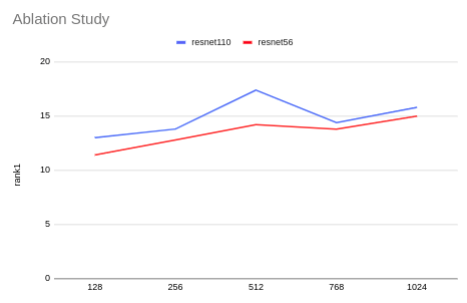
\includegraphics[scale=0.43]{img/ablation.png}
	\caption{Hasil Studi Ablasi pada \textit{Fully Connected Layer}}
	\label{fig: fclayer}
\end{figure}

Dari hasil percobaan yang dilakukan didapatkan bahwa menggunakan \textit{Fully Connected Layer} sebesar 512 mendapatkan hasil yang paling baik, dimana ketika menggunakan \textit{Fully Connected Layer} lebih dari 512 menyebabkan \textit{overfitting}. Sedangkan ketika menggunakan \textit{Fully Connected Layer} dibawah 512 tidak se-efektif menggunakan 512 layer. Gambar \ref{fig: fclayer} menunjukan grafik Rank-1 terhadap \textit{Fully Connected Layer}.

\begin{longtable}{|c|c|c|c|c|}
	\caption{Rata-rata performa semua ResNet dengan \textit{Fully Connected Layer} berbeda-beda}
	\label{tabel: 18}\\
	\hline
	\rowcolor[HTML]{C0C0C0}
	\textbf{Name} & \textbf{Rank-1} & \textbf{Rank-5} & \textbf{Rank-10} & \textbf{mAP} \\ \hline
	ResNet 56 FC 128 & 11.4\% & 36.4\% & 50\% & 15.4205\%\\ \hline
	ResNet56 FC 256 & 12.8\% & 31.8\% & 48\% & 15.71973\%\\ \hline
	ResNet 56 FC 512 & 14.2\% & 35\% & 47.8\% & 16.95365\%\\ \hline
	ResNet56 FC 768 & 13.8\% & 35.8\% & 46.8\% & 16.50338\%\\ \hline
	ResNet 56 FC 1024 & 15\% & 35.6\% & 51\% & 17.58063\%\\ \hline
	ResNet 110 FC 128 & 13\% & 35.8\% & 49\% & 15.81262\%\\ \hline
	ResNet 110 FC 256 & 13.8\% & 38.4\% & 52.8\% & 16.87966\%\\ \hline
	ResNet 110 FC 512 & 17.4\% & 38.8\% & 52.2\% & 18.87587\%\\ \hline
	ResNet 110 FC 768 & 14.4\% & 36.8\% & 48.8\% & 16.49\%\\ \hline
	ResNet 110 FC 1024 & 15.8\% & 39\% & 53.4\% & 18.0541\%\\ \hline
\end{longtable}

\begin{figure} [!htb]
	\centering
	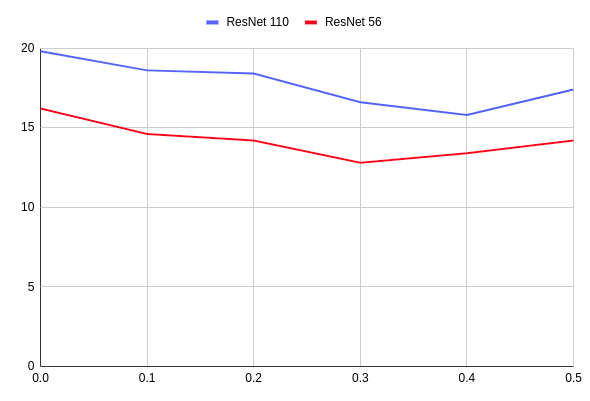
\includegraphics[scale=0.35]{img/HasilRandomErasing.png}
	\caption{Hasil Studi Ablasi pada \textit{Random Erasing}}
	\label{fig: rerasing}
\end{figure}

Sedangkan dari hasil percobaan pada \textit{Random Erasing}, didapatkan bahwa tidak menggunakan Random Erasing merupakan yang paling baik untuk model, dimana ketika menggunakan \textit{Random Erasing} performa model menurun. Sehingga ketika menggunakan Random Erasing 40\% keatas performa model menjadi tidak konsisten. Gambar \ref{fig: rerasing} menunjukan grafik Rank-1 terhadap \textit{Random Erasing}.

\section{Pengujian dengan menggunakan Ensemble}
\vspace{1ex}
Untuk meningkatkan performa dari model sendiri, dibuat sebuah ensemble dari model ResNet 56 dan ResNet 110, dimana Fully Connected layer yang digunakan sejumlah 512 layer dan tidak dilakukan Random Erasing. Selain itu dilakukan penambahan Spatial Pyramid Pooling pada ensemble dengan harapan terjadi penambahan presisi dan akurasi. Pada semua model telah dilakukan \textit{pre-training} di dataset Market 1501.

\subsection{Ensemble}
\vspace{1ex}
Pada model ini terjadi peningkatan pada Rank-1,Rank-5, Rank-10 dan mAP apabila dibandingkan dengan ResNet 110.
 
\begin{longtable}{|c|c|c|c|c|}
	\caption{Rata-rata performa ensemble }
	\label{tabel: 19}\\
	\hline
	\rowcolor[HTML]{C0C0C0}
	\textbf{No} &\textbf{Rank-1} & \textbf{Rank-5} & \textbf{Rank-10} & \textbf{mAP} \\
	\hline
	1 &24 &40 &48 &23.5601 \\
	2 &22 &40 &52 &23.8937 \\
	3 &24 &42 &60 &22.5622 \\
	4 &14 &46 &50 &18.1273 \\
	5 &26 &48 &58 &24.3952 \\
	6 &22 &44 &48 &22.6432 \\
	7 &24 &44 &50 &24.3334 \\
	8 &18 &42 &54 &21.0525 \\
	9 &14 &40 &58 &18.2236 \\
	10 &22 &38 &46 &21.7579 \\
	\hline
	\textbf{Average} & 21 & 42.4 & 52.4 &22.05491 \\
	\hline
\end{longtable}

Namun apabila dilihat dari waktu training yang dibutuhkan ensemble ini membutuhkan lebih lama dari hanya menggunakan ResNet 110.

\subsection{Ensemble + Spatial Pyramid Pooling}

\begin{longtable}{|c|c|c|c|c|}
	\caption{Rata-rata performa ensemble + Spatial Pyramid Pooling }
	\label{tabel: 20}\\
	\hline
	\rowcolor[HTML]{C0C0C0}
	\textbf{No} &\textbf{Rank-1} & \textbf{Rank-5} & \textbf{Rank-10} & \textbf{mAP} \\
	\hline
	1 &22 &44 &54 &21.425 \\
	2 &18 &44 &56 &19.6589 \\
	3 &12 &34 &48 &16.9387 \\
	4 &26 &44 &50 &23.9654 \\
	5 &16 &32 &44 &17.8318 \\
	6 &22 &48 &58 &22.1528 \\
	7 &26 &40 &52 &23.0882 \\
	8 &22 &44 &54 &21.987 \\
	9 &20 &42 &56 &21.0866 \\
	10 &18 &48 &58 &21.3644 \\
	\hline
	\textbf{Average} & 20.2 & 42 & 53 & 20.94988 \\
	\hline
\end{longtable}

Pada pengujian dengan tambahan Spatial Pyramid Pooling terjadi overfitting sehingga semua metrik evaluasi yang digunakan menurun. 

\section{Perbandingan dengan model-model lain}
\vspace{1ex}

Tabel \ref{tabel:comparison} menunjukan perbandingan performa model yang dibuat dengan model-model lain. Dari tabel tersebut dapat dilihat bahwa pada model yang dibuat Rank-1 dan Rank-5, dan Rank-10 yang didapatkan bukanlah yang terbaik.Namun pada kolom parameter dapat dilihat bahwa parameter yang dimiliki tidak sebanyak model-model lain yang pernah digunakan untuk memecahkan masalah pada dataset PKU Sketch Re-ID. Bahkan ensemble yang paling berat hanya memiliki sekitar 28.6\% parameter dari model Dense-HOG+LBP+Siamese.

\begin{longtable}{|c|c|c|c|c|}
	\caption{Perbandingan dengan model-model lain}
	\label{tabel:comparison}\\
	\hline
	\rowcolor[HTML]{C0C0C0}
			\textbf{Nama} & \textbf{Param} & \textbf{Rank-1} & \textbf{Rank-5} & \textbf{Rank-10} \\ \hline
Dense-HOG+LBP+SVM & 8.6M & 5.1\% & 16.8\% & 28.3\% \\ \hline
Triplet SN & n/a & 9\% & 26.8\% & 43.2\% \\ \hline
GN Siamese & ~14M & 28.9\% & 54\% & 62.4\%\\ \hline
Cross-Domain Adversarial & n/a & 34\% & 56.3\% & 72.5\%\\ \hline
Ensemble FC 512 & 3M & 21 \% & 42.4\% & 52.4\% \\ \hline
Ensemble SPP & 3M & 20.2\% & 42\% & 53\% \\ \hline
ResNet 110 FC 512 & 1.7M & 19.8\% & 37.4\% & 47.8\%\\ \hline
\end{longtable}



  \cleardoublepage

  % Bab 5 penutup
  \chapter{KESIMPULAN DAN SARAN}
\label{chap:penutup}

% Ubah bagian-bagian berikut dengan isi dari penutup

\section{Kesimpulan}
\label{sec:kesimpulan}

Berdasarkan hasil pengujian yang telah dilakukan dapat ditarik beberapa kesimpulan sebagai berikut:

\begin{enumerate}[nolistsep]

  \item Dikarenakan sketsa \textit{full-body} yang digunakan tidak memiliki warna, dilakukan dua percobaan untuk membantu model melakukan re-identifikasi,yaitu dengan CycleGAN dan Local Binary Pattern. Dengan menghasilkan citra sintesis dari input citra sketsa, CycleGAN meningkatkan Rank-1 \textit{accuracy} dan mAP dari model. Namun percobaan dengan {Local Binary Pattern} yang bertujuan untuk mengambil fitur tekstur dari input sketsa menyebabkan performa dari model menurun di semua metrik sehingga tidak direkomendasikan untuk digunakan.
  
  \item Untuk mengatasi kurangnya data pada PKU Sketch Re-ID, \textit{pre-training} pada dataset Market-1501 dapat meningkatkan semua metrik evaluasi dikarenakan model dapat mempelajari fitur-fitur yang terdapat pada dataset Market 1501 yang memiliki jauh lebih banyak data dibandingkan pada PKU Sketch Re-ID.
  
  \item Penggunaan \textit{Fully Connected Layer} sebesar 512 merupakan yang terbaik, apabila menggunakan \textit{Fully Connected Layer} yang lebih besar dari 512 maka akan terjadi overfitting. Namun apabila menggunakan \textit{Fully Connected Layer} dibawah 512, maka tidak se-optimal 512 layer. 
  
  \item Penggunaan \textit{Random Erasing} membuat performa model tidak konsisten, dari studi ablasi yang dilakukan lebih baik apabila tidak menggunakan \textit{Random Erasing}.
  
  \item Model yang digunakan memiliki kecepatan re-identifikasi 5 kali lebih cepat dan metrik evaluasi yang lebih baik dari DenseNet, sebuah model klasikal yang memiliki parameter lebih banyak 4 kali lipat dari ResNet CIFAR10, dan Triplet SN, sebuah model yang dibuat dari tiga model Sketch-a-Nets dan di optimisasikan dengan triplet loss.

  \item Meskipun bukan merupakan model yang terbaik, model mampu mendapatkan informasi dengan jauh lebih efisien dibandingkan model-model lain. Bahkan model ensemble, model yang paling berat pada penelitian ini, memiliki kecepatan 3 kali lebih cepat dibandingkan model DenseNet dan TripletSN.
  

\end{enumerate}

\section{Saran}
\label{chap:saran}

Untuk pengembangan lebih lanjut pada Tugas Akhir ini, terdapat beberapa saran yang dapat dilakukan, yakni sebagai berikut: 

\begin{enumerate}[nolistsep]

  \item Apabila dataset yang digunakan lebih pemasangan sketch dengan dataset membutuhkan kekuatan komputasi yang lebih besar sehingga tidak disarankan untuk menggunakan CycleGAN.
  
  \item Penggunaan Cross Domain Adversarial Learning untuk menjembatani perbedaan modalitas antara citra sketsa dengan citra CCTV.

  \item Apabila pada dataset  terdapat lebih banyak data maka \textit{pre-training} pada dataset Market 1501 tidak perlu dilakukan.

  \item Melakukan studi ablasi lebih lanjut dengan melakukan perubahan pada ukuran citra input, Random Rotation, dan Batch Size.

\end{enumerate}

  \cleardoublepage

  % Daftar pustaka
  \renewcommand\bibname{DAFTAR PUSTAKA}
  \addcontentsline{toc}{chapter}{\bibname}
  \bibliographystyle{unsrtnat}
  \bibliography{pustaka/pustaka.bib}
  \cleardoublepage

  % Biografi penulis
  \begin{center}
  \Large
  \textbf{BIOGRAFI PENULIS}
\end{center}

\addcontentsline{toc}{chapter}{BIOGRAFI PENULIS}

\vspace{2ex}

\begin{wrapfigure}{L}{0.3\textwidth}
  \centering
  \vspace{-3ex}
  % Ubah file gambar berikut dengan file foto dari mahasiswa
  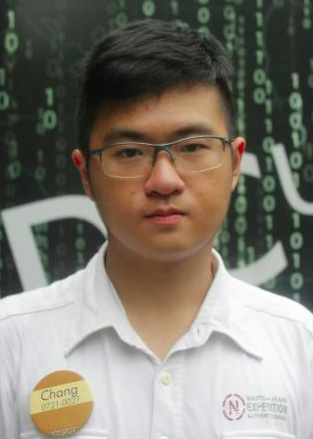
\includegraphics[width=0.3\textwidth]{gambar/chang.png}
  \vspace{-4ex}
\end{wrapfigure}

% Ubah kalimat berikut dengan biografi dari mahasiswa
\hspace{-6ex}Charles Chang atau yang lebih akrab disapa Chang, lahir di Surabaya, Jawa Timur pada 18 Agustus 1999. Merupakan anak pertama dari dua bersaudara. Penulis lulus dari SMP Kristen Petra 5 dan kemudian melanjutkan ke SMA Kristen Petra 1 Surabaya. Penulis merupakan salah satu mahasiswa dari Departemen Teknik Komputer Surabaya, Fakultas Teknologi Elektro dan Informatika Cerdas, Institut Teknologi Sepuluh Nopember. Dalam masa kuliah, penulis sangat tertarik dengan \textit{Machine Learning}, \textit{Image Processing}, dan \textit{Data Science}. Selain itu penulis juga hobi membuat permainan, dan aktif mengikuti lomba membuat permainan di masa kuliah. Bahkan pernah menjadi pemenang juara 3 di MAGE ITS, dan menjadi semi-finalis di Gemastik XII 2019.
  \cleardoublepage
  \nocite{*}
  
  

\end{document}
